\documentclass[a4paper,twoside]{article}
\usepackage[T1]{fontenc}
\usepackage[bahasa]{babel}
\usepackage{graphicx}
\usepackage{graphics}
\usepackage{float}
\usepackage[cm]{fullpage}
\pagestyle{myheadings}
\usepackage{etoolbox}
\usepackage{setspace} 
\usepackage{lipsum}
\usepackage{algorithm2e}
\setlength{\headsep}{30pt}
\usepackage[inner=2cm,outer=2.5cm,top=2.5cm,bottom=2cm]{geometry} %margin
% \pagestyle{empty}

\makeatletter
\renewcommand{\@maketitle} {\begin{center} {\LARGE \textbf{ \textsc{\@title}} \par} \bigskip {\large \textbf{\textsc{\@author}} }\end{center} }
\renewcommand{\thispagestyle}[1]{}
\markright{\textbf{\textsc{Laporan Perkembangan Pengerjaan Skripsi\textemdash Sem. Ganjil 2016/2017}}}

\onehalfspacing
 
\begin{document}

\title{\@judultopik}
\author{\nama \textendash \@npm} 

%ISILAH DATA DATA BERIKUT INI:
\newcommand{\nama}{Yohanes Mario Chandra}
\newcommand{\@npm}{2011730031}
\newcommand{\tanggal}{30/04/2017} %Tanggal pembuatan dokumen
\newcommand{\@judultopik}{Perangkat Lunak Login Otomatis \texorpdfstring{\\}{} Untuk \textit{Captive Portal} Wi-Fi} % Judul/topik anda
\newcommand{\kodetopik}{PAS4105}
\newcommand{\jumpemb}{1} % Jumlah pembimbing, 1 atau 2
\newcommand{\pembA}{Pascal Alfadian}
\newcommand{\pembB}{-}
\newcommand{\semesterPertama}{41 - Ganjil 16/17} % semester pertama kali topik diambil, angka 1 dimulai dari sem Ganjil 96/97
\newcommand{\lamaSkripsi}{2} % Jumlah semester untuk mengerjakan skripsi s.d. dokumen ini dibuat
\newcommand{\kulPertama}{Skripsi 1} % Kuliah dimana topik ini diambil pertama kali
\newcommand{\tipePR}{C} % tipe progress report :
% A : dokumen pendukung untuk pengambilan ke-2 di Skripsi 1
% B : dokumen untuk reviewer pada presentasi dan review Skripsi 1
% C : dokumen pendukung untuk pengambilan ke-2 di Skripsi 2
\maketitle

\pagenumbering{arabic}

\section{Data Skripsi} %TIDAK PERLU MENGUBAH BAGIAN INI !!!
Pembimbing utama/tunggal: {\bf \pembA}\\
Pembimbing pendamping: {\bf \pembB}\\
Kode Topik : {\bf \kodetopik}\\
Topik ini sudah dikerjakan selama : {\bf \lamaSkripsi} semester\\
Pengambilan pertama kali topik ini pada : Semester {\bf \semesterPertama} \\
Pengambilan pertama kali topik ini di kuliah : {\bf \kulPertama} \\
Tipe Laporan : {\bf \tipePR} -
\ifdefstring{\tipePR}{A}{
			Dokumen pendukung untuk {\BF pengambilan ke-2 di Skripsi 1} }
		{
		\ifdefstring{\tipePR}{B} {
				Dokumen untuk reviewer pada presentasi dan {\bf review Skripsi 1}}
			{	Dokumen pendukung untuk {\bf pengambilan ke-2 di Skripsi 2}}
		}

\section{Detail Perkembangan Pengerjaan Skripsi}
Detail bagian pekerjaan skripsi sesuai dengan rencan kerja/laporan perkembangan terkahir :
	\begin{enumerate}
		\item Melakukan studi literatur mengenai hal-hal yang berkaitan dengan perancangan dan pembuatan apli-
kasi.\\
		{\bf status :} Ada sejak rencana kerja skripsi.\\
		{\bf hasil :} Sudah dilakukan studi literatur. \textit{Captive Portal}: \textit{router} atau \textit{gateway} yang akan menutup koneksi eksternal sampai klien yang bersangkutan sudah terotentikasi. Protokol HTTP mengatur kode status yang dapat digunakan untuk mengindikasikan adanya \textit{captive portal}, yaitu kode status 511. \textit{.NET Framework}: platform yang bersifat \textit{general purpose} untuk membangun aplikasi. \textit{.NET Framework} memanfaatkan \textit{Common Language Infrastructure} untuk memberikan kebebasan kepada \textit{developer} untuk memilih bahasa yang ingin digunakan selama bahasa tersebut didukung oleh \textit{.NET Framework}. \textit{Universal Windows Platform} (UWP): arsitektur aplikasi umum untuk Windows. Memungkinkan aplikasi dapat dijalankan pada desktop dan Windows Phone. Kelas WebBrowser tidak jadi dipelajari, karena UWP tidak mendukung WebBrowser. Oleh karena itu, dipelajari kelas WebView. WebView memungkinkan developer untuk menampung konten HTML pada suatu aplikasi. WebView tidak mendukung masukkan pengguna seperti key-down, key-up, dan pointer-pressed. Oleh karena itu, dibutuhkan metode lain yang melibatkan InvokeScriptAsync dengan fungsi eval javascript untuk menggunakan HTML event handler dan fungsi window.external.notify untuk menangani event dari HTML pada aplikasi. PasswordVault: kelas yang merepresentasikan pengunci kredensial.  Kredensial yang disimpan menggunakan kelas ini hanya dapat diakses oleh aplikasi atau service yang bersangkutan.
		
		\item Melakukan analisis perangkat lunak sejenis.\\
		{\bf status :} Ada sejak rencana kerja skripsi.\\
		{\bf hasil :} Perangkat lunak sejenis pada Windows belum dapat ditemukan pada saat penelitian ini dilakukan. Oleh karena itu, perangkat lunak atau aplikasi sejenis yang dianalisis adalah aplikasi yang diciptakan untuk sistem operasi Android. Aplikasi tersebut bernama \textit{WiFi Web Login}. Langkah-langkah yang harus ditempuh untuk melakukan \textit{login} wifi berbasis web pada aplikasi ini adalah:

\begin{enumerate}
    \item{Deteksi sambungan dengan wifi yang bersangkutan.}
    \item{Deteksi hubungan dengan internet.}
    \item{Jika tidak terjadi hubungan dengan internet, deteksi apakah tersimpan informasi login untuk wifi yang bersangkutan.}
    \item{Jika terdapat informasi login untuk wifi yang bersangkutan maka lakukan login otomatis.}
    \item{Jika tidak terdapat informasi login untuk wifi yang bersangkutan maka rekam informasi login dan lakukan login.}
\end{enumerate}

Setelah pengguna melalui sudah pernah melakukan login pertama kali menggunakan aplikasi tersebut, maka aplikasi akan melakukan login otomatis setiap kali terhubung dengan wifi yang bersangkutan.

		\item  Melakukan analisis kebutuhan untuk mengimplementasikan mekanisme login otomatis ini\\
		{\bf status :} Ada sejak rencana kerja skripsi.\\
		{\bf hasil :} Ada beberapa metode yang diperlukan untuk mengimplementasikan mekanisme login otomatis:
        \begin{itemize}
            \item{
                Metode Penyimpanan Informasi Login
                
                Penyimpanan informasi login dapat dilakukan dengan beberapa metode, diantaranya adalah dengan menggunakan file teks atau menggunakan PasswordVault. Penyimpanan informasi menggunakan file teks berarti informasi disimpan dalam bentuk \textit{plaintext} dalam file yang diberikan \textit{access permission} tertentu. Sementara itu, penyimpanan informasi menggunakan PasswordVault memanfaatkan kelas API yang terdapat pada \textit{Universal Windows Platform} (UWP).
                
                Informasi yang perlu disimpan untuk dapat melakukan login otomatis adalah \textit{connection fingerprint} (seperti SSID WiFi, url, dan potongan unik dokumen html), username, password, dan langkah-langkah login seperti menekan tombol. Oleh karena itu, metode penyimpanan menggunakan credential locker dan file teks perlu dianalisis untuk dapat ditentukan metode mana yang paling cocok untuk digunakan dalam penelitian ini.
                
                PasswordVault dapat menyimpan informasi yang berisi \textit{resource} (biasanya berupa nama aplikasi atau string unik lainnya), username, dan password. Informasi yang perlu disimpan selain username dan password adalah \textit{connection fingerprint} dan langkah-langkah login. \textit{Connection fingerprint} dapat disimpan pada resource karena sifatnya yang unik. Sementara itu, langkah-langkah login dapat disimpan pada username atau password karena langkah-langkah login dapat disimpan dalam bentuk String. Akan tetapi, langkah-langkah login sebaiknya disimpan pada password, dipisahkan dengan karakter pemisah tertentu, agar username dapat digunakan sebagai \textit{identifier} unik. PasswordVault memiliki batasan 10 kredensial yang dapat disimpan per aplikasi. Jika aplikasi mencoba menyimpan lebih dari 10 kredensial maka akan terjadi exception. Oleh karena hal ini, PasswordVault menjadi pilihan yang kurang baik untuk kebutuhan perangkat lunak pada penelitian ini.

                Metode penyimpanan lainnya adalah dengan menggunakan file teks. Penyimpanan informasi mengunakan file teks dapat dilakukan untuk informasi berbasis teks apapun dan tidak ada batasan banyaknya informasi yang dapat disimpan (kecuali batasan perangkat keras seperti kapasitas hard disk). Akan tetapi, file teks dapat dibaca oleh aplikasi manapun, sehingga penyimpanan informasi sensitif tidak dapat dilakukan tanpa adanya metode pengamanan tertentu. Salah satu metode pengamanan yang dapat dilakukan adalah dengan mendeklarasikan \textit{file access permission}. Akan tetapi, karena Windows memiliki \textit{security model} per pengguna dan bukan per aplikasi, maka aplikasi lain yang dijalankan oleh pengguna tersebut memiliki akses yang sama kepada file yang bersangkutan. Metode pengamanan lainnya adalah dengan melakukan enkripsi pada file yang bersangkutan sehingga hanya pemegang kunci yang dapat membaca file tersebut. Enkripsi file pada windows dapat dilakukan menggunakan kelas CryptographicEngine. Kunci enkripsi dan dekripsi dapat disimpan menggunakan PasswordVault atau dengan meminta pengguna untuk memasukkan kunci tersebut setiap kali aplikasi dijalankan.

                Metode penyimpanan yang digunakan pada penelitian ini adalah metode penyimpanan menggunakan file teks. Akan tetapi, seperti yang sudah dijabarkan sebelumnya, diperlukan metode pengamanan untuk file teks tersebut. Metode pengamanan yang digunakan adalah enkripsi file teks yang bersangkutan. Kunci enkripsi dan dekripsi dibangun secara random saat aplikasi pertama kali dijalankan dan disimpan menggunakan PasswordVault.
            }
            \item{
                Metode Rekam dan Kirim Informasi Login
                
                Kelas WebView pada \textit{Universal Windows Platform} (UWP) hanya dapat dihubungkan dengan kode C\# menggunakan javascript. \textit{Method} yang digunakan untuk melakukan eksekusi javascript pada WebView adalah InvokeScriptAsync. Metode ini memiliki parameter string berupa nama fungsi javascript yang ingin dipanggil dan array of string yang berisi argumen yang ingin dikirimkan ke dalam fungsi tersebut. Salah satu fungsi yang dapat dipanggil adalah \textit{eval}. Dengan menggunakan \textit{eval}, ekspresi javascript apapun dapat dijalankan pada WebView. Untuk mengirimkan data dari javascript ke kode C\#, dapat dijalankan fungsi window.external.notify dengan parameter berupa string. Oleh karena itu, diperlukan \textit{encoding} tertentu (seperti JSON\footnote{https://tools.ietf.org/html/rfc7159}) untuk memasukkan lebih dari satu argumen.

                InvokeScriptAsync dapat digunakan untuk memanggil fungsi \textit{eval} dengan parameter berupa function yang dapat digunakan untuk menekan tombol atau memasukkan nilai pada \textit{text field} tertentu. Selain itu, dapat dimasukkan event listener yang dapat memanggil window.external.notify menggunakan cara ini. Fungsi window.external.notify dapat membantu mengirimkan event-event seperti mouse click, keypress, atau perubahan nilai pada \textit{text field} yang ada pada halaman HTML pada WebView tersebut.
            }
            \item{
                Metode Deteksi \textit{Captive Portal}
                
                Kode status HTTP 511 digunakan untuk memberitahu klien bahwa respon yang didapat bukan berasal dari server tujuan dan diperlukan otentikasi jaringan. Akan tetapi, pada prakteknya, tidak semua \textit{captive portal} melakukan implementasi kode status HTTP 511.
                
                \textit{Captive portal} milik Unpar mengirimkan kode status 302, dan bukan 511. Oleh karena adanya perbedaan implementasi seperti ini, deteksi \textit{captive portal} menggunakan kode status HTTP tidak dapat dilakukan.
                
                Persamaan implementasi yang dimiliki oleh setiap \textit{captive portal} adalah dibutuhkannya \textit{redirection} yang dapat dikenali oleh \textit{web browser} agar klien selalu diarahkan ke halaman \textit{captive portal} tersebut sebelum melakukan otentikasi. Oleh karena itu, untuk setiap HTTP \textit{request} yang dilakukan oleh klien sebelum melakukan otentikasi, HTTP \textit{response} yang diberikan bukanlah berasal dari server tujuan. Sifat ini dapat dimaanfaatkan untuk keperluan deteksi \textit{captive portal} dengan mengirimkan \textit{request} ke server yang sudah ditentukan sebelumnya, dan mendeteksi apakah \textit{response} yang diberikan sesuai dengan harapan. Jika \textit{response} yang diberikan tidak sesuai dengan harapan, maka dapat diasumsikan bahwa klien dibatasi oleh suatu \textit{captive portal}.

                Kelas WebView pada \textit{Universal Windows Platform} (UWP) memiliki kemampuan deteksi \textit{redirection} dan \textit{response} yang tidak sesuai harapan seperti \textit{web browser} pada umumnya. Oleh karena itu, kelas WebView digunakan untuk melakukan deteksi \textit{captive portal} pada penelitian ini tanpa perlu memeriksa kode status HTTP setiap \textit{response}. Penggunaan kelas WebView juga akan mempermudah proses otomatisasi login karena WebView dapat melakukan hal-hal yang dapat dilakukan oleh \textit{web browser} pada umumnya seperti menjalankan javascript dan menampilkan halaman HTML.
            }
        \end{itemize}
        
        \pagebreak
        
        Diagram \textit{Use Case}:
        
        \begin{figure}[h]
            \centering
            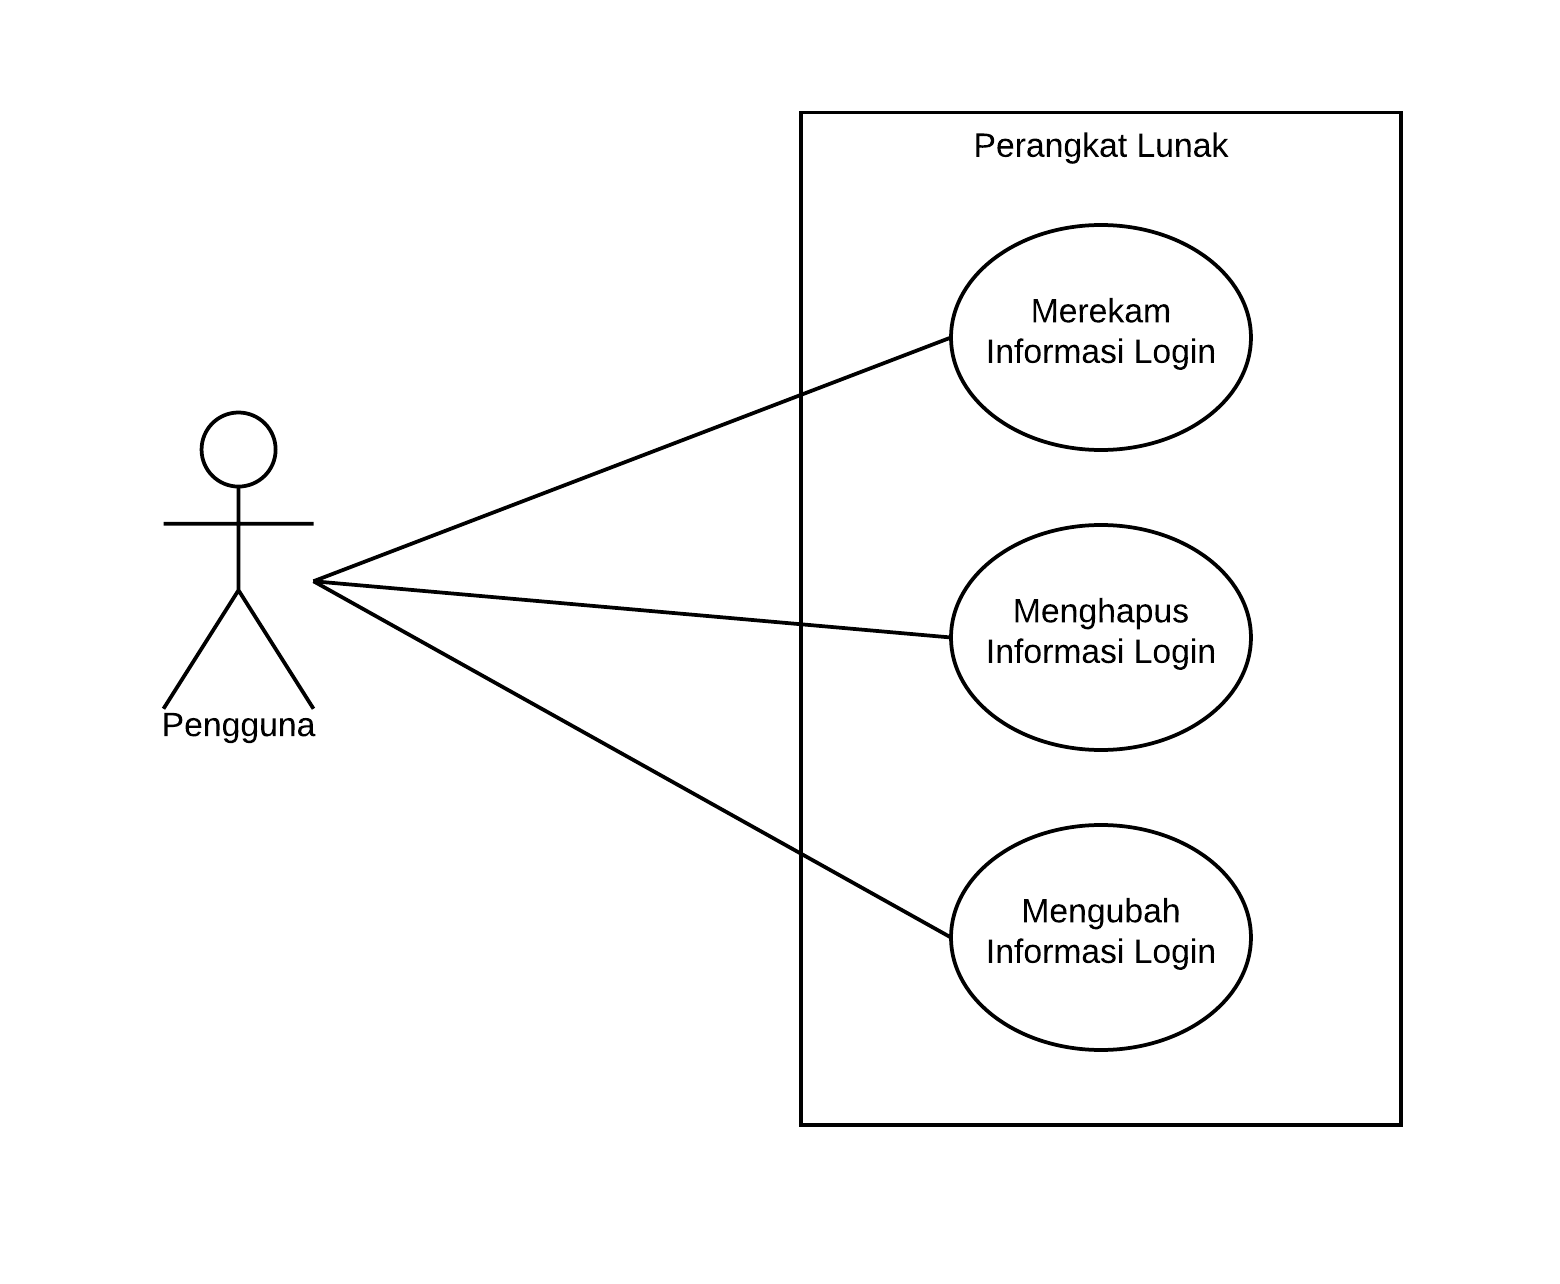
\includegraphics[scale=0.77]{usecase.png}
            \caption[Diagram \textit{use case} untuk perangkat lunak yang dibangun.]{Diagram \textit{use case} untuk perangkat lunak yang dibangun.}
            \label{fig:usecase}
        \end{figure}

        \textbf{Skenario merekam informasi login}\\
        Nama: Merekam informasi login\\
        Aktor: Pengguna\\
        Kondisi awal: Perangkat lunak mendeteksi adanya \textit{captive portal}.\\
        Deskripsi: Pengguna menyimpan informasi login.\\
        Kondisi Akhir: Informasi login tersimpan di dalam perangkat lunak.\\
        Skenario:
        \begin{enumerate}
            \item{Pengguna memasukkan informasi login ke dalam form HTML.}
            \item{Sistem menyimpan informasi login yang dimasukkan oleh pengguna.}
        \end{enumerate}

        \textbf{Skenario menghapus informasi login}\\
        Nama: Menghapus informasi login\\
        Aktor: Pengguna\\
        Kondisi awal: Perangkat lunak sudah dijalankan.\\
        Deskripsi: Pengguna menghapus informasi login.\\
        Kondisi Akhir: Informasi login dihapus dari perangkat lunak.\\
        Skenario:
        \begin{enumerate}
            \item{Pengguna memilih untuk menghapus informasi login.}
            \item{Sistem menghapus informasi login.}
        \end{enumerate}

        \textbf{Skenario mengubah informasi login}\\
        Nama: Mengubah informasi login\\
        Aktor: Pengguna\\
        Kondisi awal: Perangkat lunak sudah dijalankan.\\
        Deskripsi: Pengguna mengubah informasi login.\\
        Kondisi Akhir: Informasi login diubah dari perangkat lunak.\\
        Skenario:
        \begin{enumerate}
            \item{Pengguna memilih untuk mengubah informasi login.}
            \item{Sistem menampilkan form ubah informasi login.}
            \item{Pengguna memasukkan informasi login baru.}
            \item{Sistem menghapus informasi login lama dan menyimpan informasi login baru.}
        \end{enumerate}

        \textbf{Skenario memicu login otomatis}\\
        Nama: Memicu login otomatis\\
        Aktor: WiFi\\
        Kondisi awal: Perangkat lunak sudah dijalankan.\\
        Deskripsi: Sistem memicu login otomatis berdasarkan perubahan status WiFi.\\
        Kondisi Akhir: Klien terotentikasi pada \textit{captive portal}.\\
        Skenario:
        \begin{enumerate}
            \item{Sistem mendeteksi adanya koneksi WiFi yang terjadi.}
            \item{Sistem mendeteksi adanya \textit{captive portal}.}
            \item{Sistem mendeteksi adanya informasi login untuk \textit{captive portal} tersebut.}
            \item{Sistem mengirimkan informasi login kepada \textit{captive portal}.}
            \item{Sistem mendeteksi koneksi dengan internet dan klien sudah terotentikasi pada \textit{captive portal} tersebut.}
        \end{enumerate}
        
        Diagram Kelas:
        
        \begin{figure}[h]
            \centering
            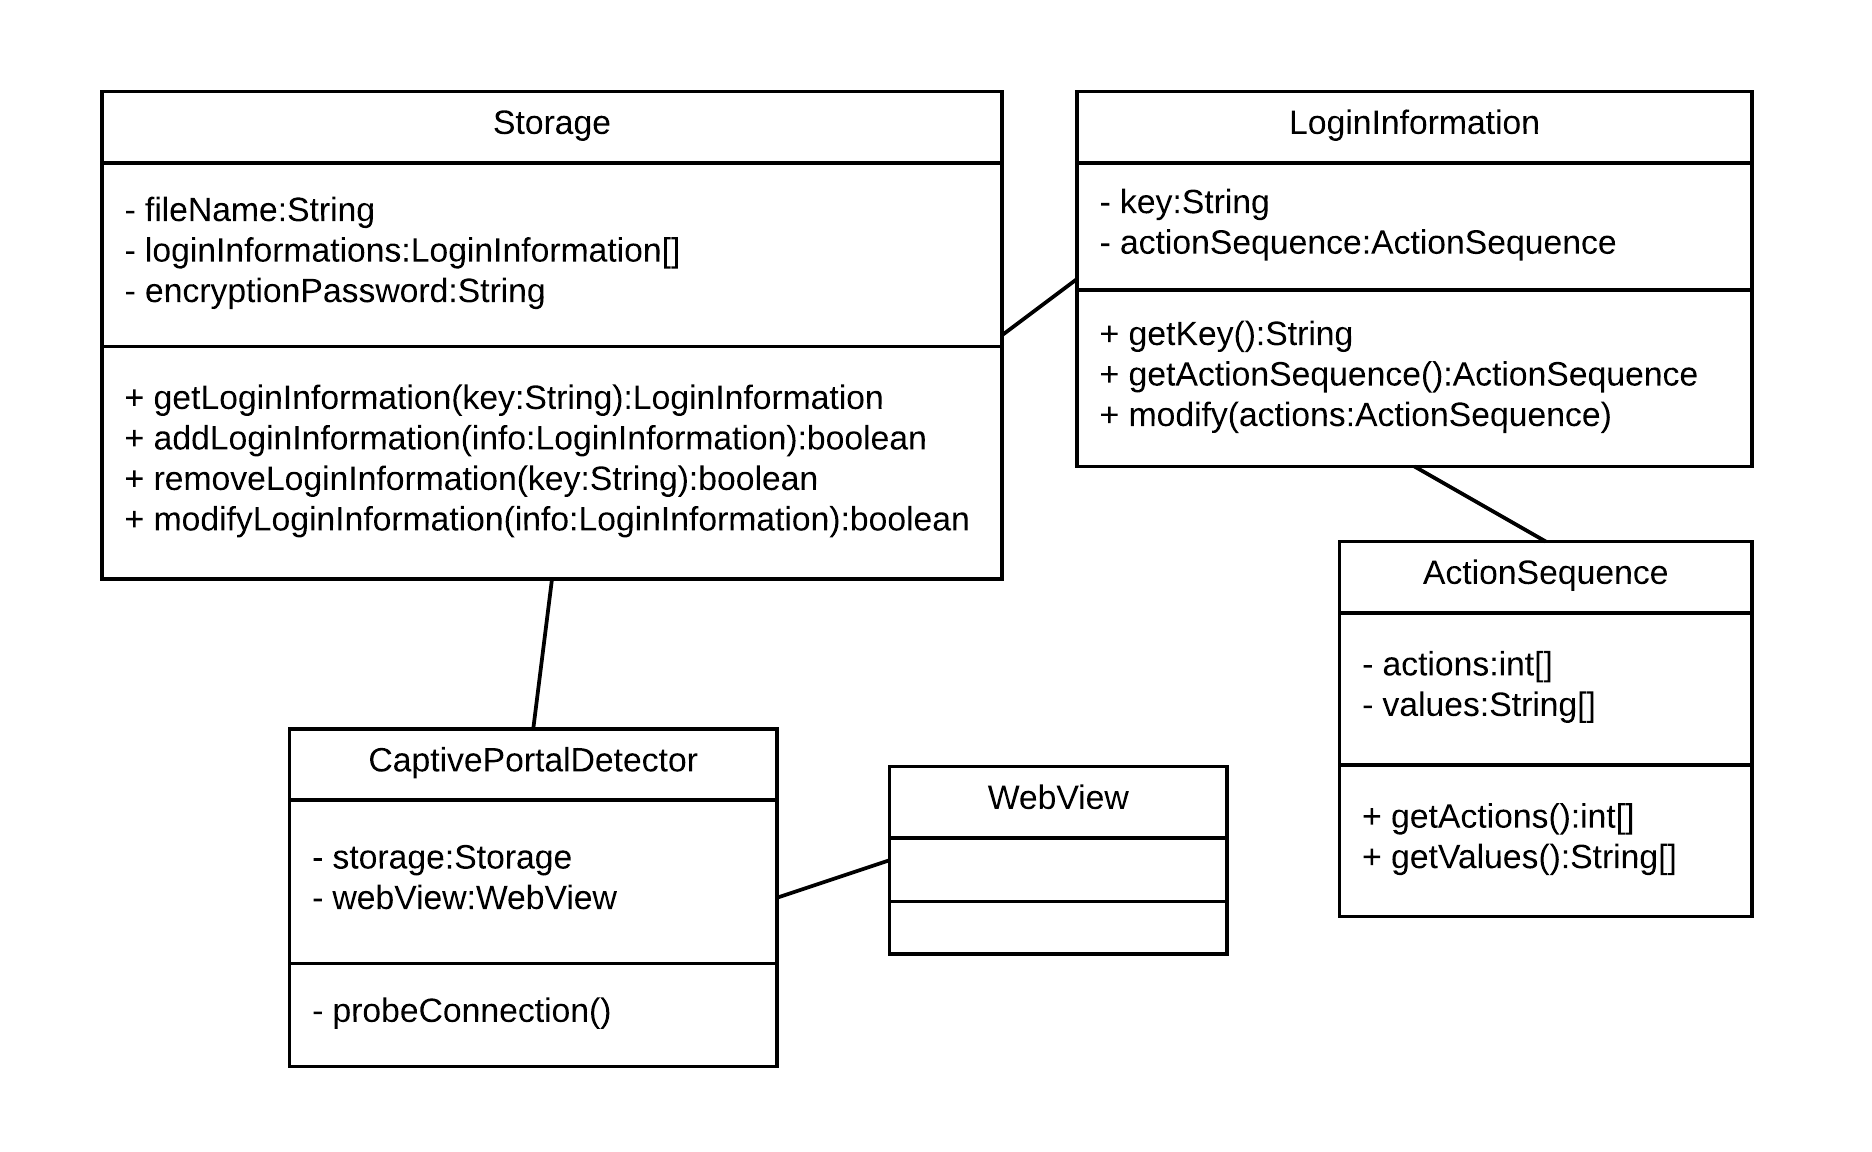
\includegraphics[scale=0.85]{classdiagram.png}
            \caption[Diagram kelas untuk perangkat lunak yang dibangun.]{Diagram kelas untuk perangkat lunak yang dibangun.}
            \label{fig:diagramkelas}
        \end{figure}
        
        Kelas-kelas yang dibutuhkan pada perangkat lunak ini adalah:
        
        \begin{itemize}
            \item{CaptivePortalDetector\\Kelas ini digunakan untuk mendeteksi keberadaan \textit{captive portal}. Jika captive portal terdeteksi, maka informasi login yang tersimpan dalam Storage digunakan. Jika tidak terdapat informasi login dalam Storage, maka direkam informasi login baru.}
            \item{Storage\\Kelas ini digunakan untuk menyimpan seluruh informasi login dalam bentuk file teks yang sudah terenkripsi.}
            \item{LoginInformation\\Kelas ini digunakan untuk menyimpan informasi login dalam bentuk key atau fingerprint, serta ActionSequence}
            \item{ActionSequence\\Kelas ini digunakan untuk menyimpan langkah-langkah login dalam bentuk urutan aksi dan nilai-nilai yang berkaitan dengan aksi tersebut.}
        \end{itemize}

		\item Merancang perangkat lunak login otomatis ini\\
		{\bf status :} Ada sejak rencana kerja skripsi.\\
		{\bf hasil :} Perancangan yang dilakukan mencakupi perancangan kelas, diagram \textit{sequence}, serta penjelasan mengenai hasil analisis yang tidak mungkin diimplementasikan dan cara lain yang dilakukan untuk mendapatkan hasil yang serupa.
        \begin{itemize}
            \item{
                {\bf Perancangan Kelas}\\
                Gambar \ref{fig:DetailedClassDiagram} menjelaskan mengenai kelas-kelas dalam perangkat lunak yang dibuat. Beberapa kelas utama yang perlu dijelaskan antara lain:\\
                \textbf{MainPage} : Kelas ini merupakan kelas yang berperan sebagai tampilan utama aplikasi. Atribut-atribut yang dimiliki oleh kelas ini adalah:
                \begin{itemize}
                    \item{cpd\\Atribut untuk menyimpan \textit{instance} CaptivePortalDetector.}
                    \item{timeoutTimer\\Atribut untuk menyimpan timer yang digunakan untuk menghitung \textit{connection timeout}.}
                    \item{loaded\\Atribut untuk menyimpan status \textit{loading} suatu halaman.}
                \end{itemize}
                Metode-metode yang dimiliki oleh kelas ini adalah:
                \begin{itemize}
                    \item{setup\\Metode ini digunakan untuk melakukan \textit{setup} awal saat aplikasi dieksekusi. Fungsinya adalah untuk menyimpan \textit{instance} CaptivePortalDetector dan memanggil metode setup() pada \textit{instance} tersebut.}
                    \item{MainWebView\_LoadCompleted\\Metode ini dipanggil saat WebView selesai melakukan loading halaman. Fungsinya adalah untuk memanggil metode onLoad() pada CaptivePortalDetector.}
                    \item{MainWebView\_NavigationStarting\\Metode ini dipanggil saat WebView baru akan memulai navigasi ke halaman baru. Fungsinya adalah untuk memulai \textit{timer} untuk \textit{timeout} dan memasukkan objek ScriptNotifyHandler.}
                    \item{MainWebView\_NewWindowRequested\\Metode ini dipanggil saat WebView melakukan \textit{request} untuk membuka window baru. Fungsinya adalah untuk memanggil metode queueUri() pada CaptivePortalDetector.}
                    \item{MainWebView\_NavigationCompleted\\Metode ini dipanggil saat WebView selesai melakukan navigasi ke halaman baru, namun belum selesai melakukan loading halaman tersebut. Fungsinya adalah untuk melakukan \textit{override} fungsi-fungsi JavaScript seperti window.open() dan open() agar bisa diakses dari JavaScript tanpa aksi langsung dari pengguna.}
                \end{itemize}
                
                \textbf{NetChangeDetectorBackgroundTask} : Kelas ini merupakan kelas yang digunakan untuk melakukan deteksi perubahan jaringan yang nantinya digunakan untuk menampilkan notifikasi apabila terdeteksi adanya jaringan yang terhubung tanpa adanya internet. Atribut yang dimiliki oleh kelas ini adalah:
                \begin{itemize}
                    \item{lastSSID\\Atribut ini menyimpan SSID terakhir yang nantinya akan dibandingkan dengan SSID terbaru untuk mendeteksi adanya perubahan SSID.}
                \end{itemize}
                Metode-metode yang dimiliki oleh kelas ini adalah:
                \begin{itemize}
                    \item{Run\\Metode ini dipanggil saat Windows mengalami perubahan jaringan. Fungsinya adalah untuk menampilkan notifikasi apabila kondisi \texttt{connectionChanged() \&\& lastSSID!=null \&\& hasNoInternetAccess()} terpenuhi.}
                    \item{hasNoInternetAccess\\Metode ini digunakan untuk medeteksi tidak adanya akses internet menggunakan API yang diberkan oleh UWP.}
                    \item{conectionChanged\\Metode ini digunakan untuk medeteksi perubahan SSID.}
                \end{itemize}
                
                \textbf{ScriptNotifyHandler} : Kelas ini merupakan kelas yang digunakan untuk menghubungkan sisi javascript pada WebView dengan kode C\#. Metode-metode yang dimiliki oleh kelas ini adalah:
                \begin{itemize}
                    \item{passAction\\Metode ini dipanggil saat \textit{listener} yang sudah disisipkan ke dalam WebView mendeteksi \textit{action} yang dapat direkam. \textit{Action} yang direkam berupa teks yang berisi kode javascript yang dapat mereplikasi \textit{action} tersebut.}
                    \item{windowOpen\\Metode ini dipanggil saat javascript pada WebView memanggil fungsi window.open atau fungsi open.}
                \end{itemize}
                
                \textbf{CaptivePortalDetector} : Kelas ini merupakan kelas utama yang berfungsi untuk melakukan deteksi \textit{captive portal}, menyisipkan kode \textit{listener} pada WebView, merekam \textit{action sequence} yang dilakukan oleh pengguna, dan menjalankan kembali \textit{action sequence} yang sudah tersimpan. Kelas ini menggunakan \textit{design pattern} singleton agar kelas-kelas lainnya bisa mengakses \textit{instance} yang sama pada setiap \textit{session}. Atribut yang dimiliki oleh kelas ini adalah:
                \begin{itemize}
                    \item{instance\\Atribut ini menyimpan \textit{instance} CaptivePortalDetector.}
                    \item{storage\\Atribut ini menyimpan objek Storage yang digunakan untuk menyimpan dan mengakses informasi login.}
                    \item{ssid\\Atribut ini menyimpan SSID saat ini.}
                    \item{uriQueue\\Atribut ini menyimpan queue Uri yang perlu diakses.}
                    \item{webView\\Atribut ini menyimpan WebView yang digunakan untuk melakukan deteksi \textit{captive portal}.}
                    \item{textBlock\\Atribut ini menyimpan TextBlock yang digunakan untuk menampilkan pesan kepada pengguna.}
                    \item{comboBox\\Atribut ini menyimpan ComboBox yang digunakan untuk menampilkan daftar SSID yang sudah tersimpan kepada pengguna.}
                    \item{currentFingerprint\\Atribut ini menyimpan fingerprint saat ini.}
                    \item{currentActionSequence\\Atribut ini menyimpan ActionSequence yang terkait dengan fingerprint saat ini.}
                    \item{timer\\Atribut ini menyimpan timer yang digunakan untuk mengatur waktu akses Uri dalam uriQueue.}
                \end{itemize}
                Metode-metode yang dimiliki oleh kelas ini adalah:
                \begin{itemize}
                    \item{getInstance\\Metode ini digunakan untuk mendapatkan \textit{instance} dari CaptivePortalDetector.}
                    \item{setup\\Metode ini digunakan untuk melakukan \textit{setup} awal yang menyimpan WebView, TextBlock, dan ComboBox ke dalam \textit{instance} CaptivePortalDetector.}
                    \item{refreshList\\Metode ini digunakan untuk melakukan \textit{refresh} tampilan ComboBox.}
                    \item{updateWebView\\Metode ini digunakan untuk menentukan melakukan deteksi \textit{captive portal} jika terhubung dengan koneksi WiFi, atau menampilkan pesan kepada pengguna juka tidak terhubung dengan koneksi WiFi.}
                    \item{onLoad\\Metode ini dipanggil saat WebView sudah selesai melakukan \textit{loading} halaman. Fungsinya adalah untuk melakukan deployListener(), menjalankan aksi-aksi yang sudah terekam pada informasi login, dan mendeteksi sudah atau belum terjadinya koneksi dengan internet.}
                    \item{navigationStarting\\Metode ini dipanggil saat WebView mulai melakukan navigasi ke halaman baru. Fungsinya adalah untuk membatalkan timer untuk membuka halaman-halaman popup dari halaman sebelumnya.}
                    \item{passAction\\Metode ini digunakan untuk menyimpan \textit{action} yang dikirimkan oleh ScriptNotifyHandler ke dalam currentActionSequence.}
                    \item{updateSSID\\Metode ini digunakan untuk mendapatkan SSID terbaru.}
                    \item{queueUri\\Metode ini digunakan untuk memasukkan Uri baru ke dalam uriQueue.}
                    \item{timeout\\Metode ini digunakan untuk menyatakan bahwa terjadi \textit{connection timeout}.}
                    \item{removeLoginInformation\\Metode ini digunakan untuk menghapus seluruh informasi login yang terkait dengan SSID tertentu.}
                \end{itemize}
                
                \textbf{Storage} : Kelas ini digunakan untuk menyimpan informasi login dan password yang digunakan untuk melakukan enkripsi. Atribut yang dimiliki oleh kelas ini adalah:
                \begin{itemize}
                    \item{fileName\\Atribut ini menyimpan nama file yang digunakan untuk menyimpan informasi login yang terenkripsi.}
                    \item{password\\Atribut ini menyimpan password yang digunakan untuk melakukan enkripsi.}
                    \item{loginInfo\\Atribut ini menyimpan objek LoginInformation yang digunakan untuk menyimpan seluruh informasi login.}
                \end{itemize}
                Metode-metode yang dimiliki oleh kelas ini adalah:
                \begin{itemize}
                    \item{setup\\Metode ini digunakan untuk melakukan \textit{setup} awal seperti membuka file dan melakukan dekripsi.}
                    \item{getLoginInfo\\Metode ini digunakan untuk mendapatkan objek LoginInformation.}
                    \item{saveData\\Metode ini digunakan untuk menyimpan data yang ada pada objek LoginInformation ke dalam file dan melakukan enkripsi pada file tersebut.}
                \end{itemize}
                
                \textbf{LoginInformation} : Kelas ini digunakan untuk merepresentasikan informasi login. Atribut yang dimiliki oleh kelas ini adalah:
                \begin{itemize}
                    \item{actionSequences\\Atribut ini merupakan pasangan \textit{key-value} antara suatu fingerprint dengan ActionSequence.}
                \end{itemize}
                Metode-metode yang dimiliki oleh kelas ini adalah:
                \begin{itemize}
                    \item{getActionSequence\\Metode ini digunakan untuk mendapatkan ActionSequence berdasarkan fingerprint tertentu.}
                    \item{addActionSequence\\Metode ini digunakan untuk menambahkan ActionSequence untuk fingerprint tertentu.}
                    \item{removeBySSID\\Metode ini digunakan untuk menghapus ActionSequence milik fingerprint tertentu.}
                    \item{getList\\Metode ini digunakan untuk mendapatkan daftar SSID yang sudah direkam.}
                \end{itemize}
                
                \textbf{ActionSequence} : Kelas ini digunakan untuk merepresentasikan urutan \textit{action}. Atribut yang dimiliki oleh kelas ini adalah:
                \begin{itemize}
                    \item{actions\\Atribut ini merupakan daftar \textit{action} yang berupa kode javascript.}
                \end{itemize}
                Metode-metode yang dimiliki oleh kelas ini adalah:
                \begin{itemize}
                    \item{add\\Metode ini digunakan untuk menambahkan \textit{action} ke dalam daftar ini.}
                    \item{getEnumerable\\Metode ini digunakan untuk mendapatkan enumerable dari daftar \textit{actions}, sehingga mempermudah eksekusi \textit{actions}.}
                    \item{reset\\Metode ini digunakan untuk menghapus seluruh \textit{action} yang ada pada daftar ini.}
                \end{itemize}
                
                \begin{figure}[!htb]
                    \centering
                    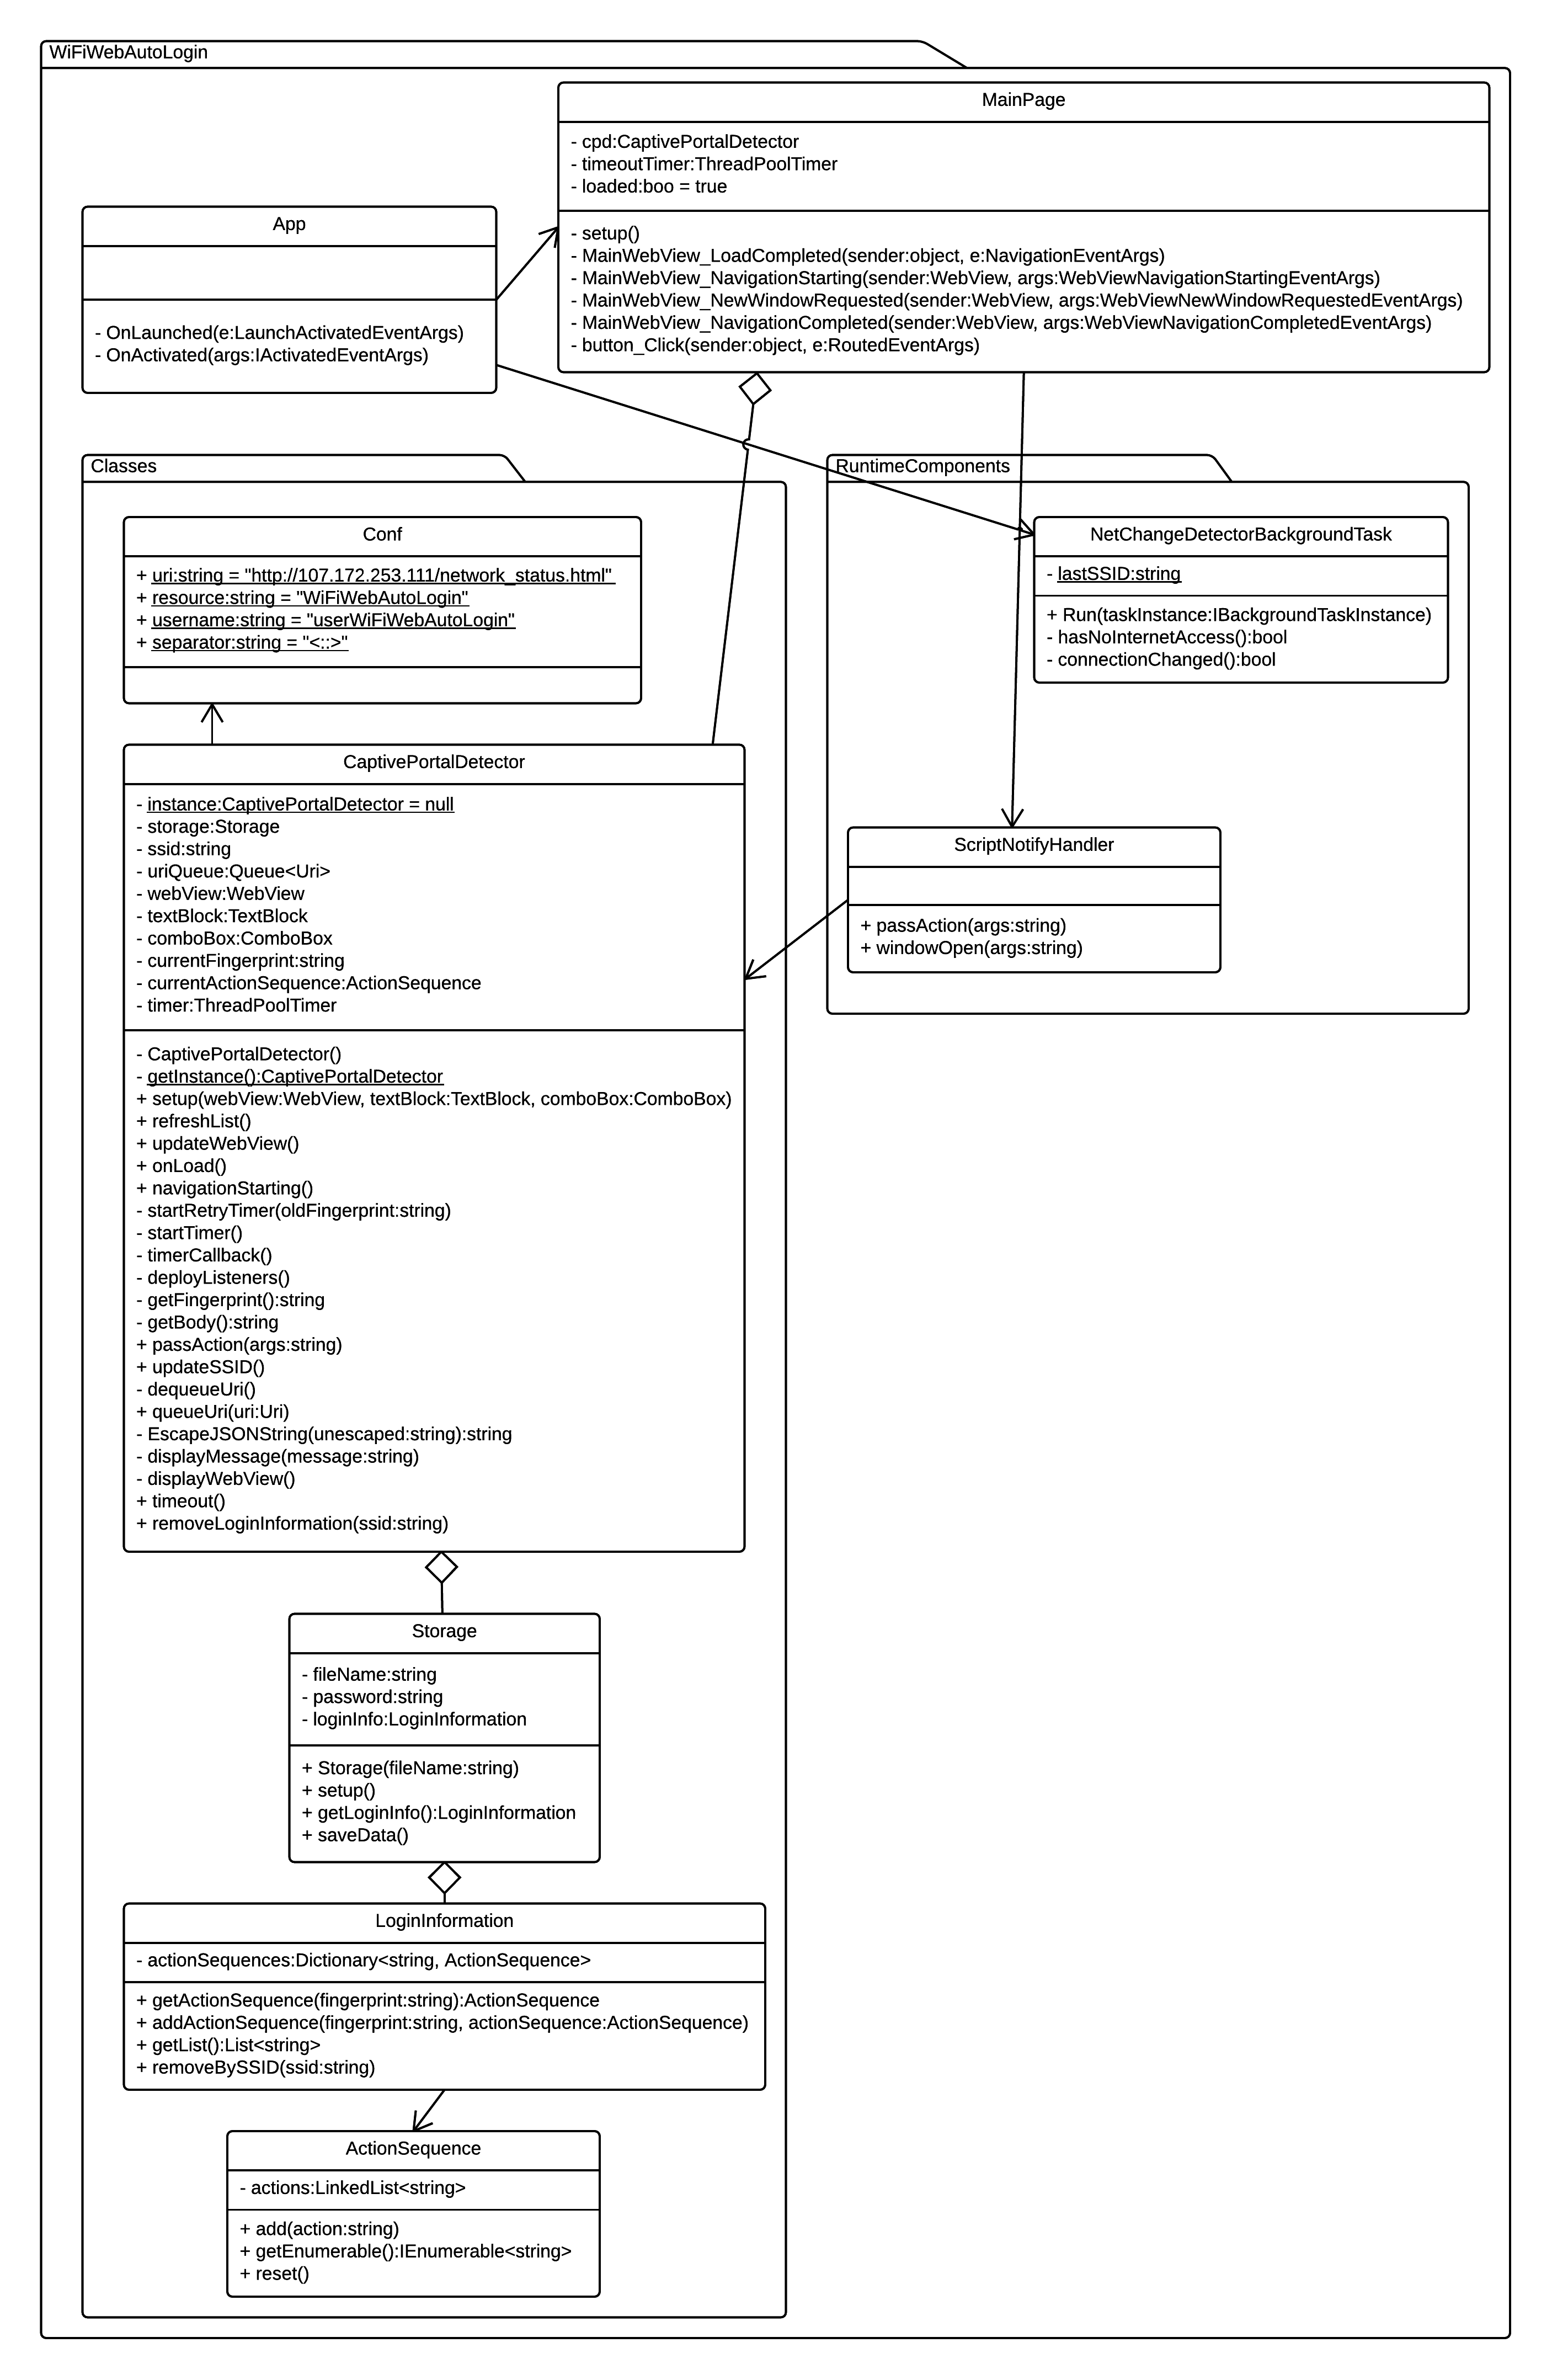
\includegraphics[scale=0.63]{DetailedClassDiagram.png}
                    \caption[Diagram Kelas Rinci.]{Diagram Kelas Rinci.} 
                    \label{fig:DetailedClassDiagram}
                \end{figure}
            }
            \item{
                {\bf Perancangan Algoritma dan Struktur Data}
                \begin{itemize}
                    \item{
                        {\bf Algoritma Deteksi \textit{Captive Portal}}\\
                        Algoritma yang digunakan untuk melakukan deteksi \textit{captive portal} adalah sebagai berikut:

                        \hfill

                        \begin{algorithm}[H]
                            \If{Network Detected and No Internet Connection}{
                                Ask user to run application via notification\;
                                \If{"Yes" button clicked}{
                                    Access a web page which can only be opened if there is an internet connection\;
                                    \If{Redirected}{
                                        Captive portal detected\;
                                    }
                                }
                            }
                        \end{algorithm}

                        \hfill

                        Algoritma di atas menjelaskan deteksi \textit{captive portal} dilakukan dengan melakukan deteksi jaringan yang tidak terhubung dengan internet. Jika ditemukan jaringan yang tidak terhubung dengan internet, maka akan muncul notifikasi yang memungkinkan pengguna untuk menjalankan perangkat lunak. Saat perangkat lunak dijalankan, perangkat lunak akan mencoba untuk mengakses halaman pancingan yang beralamatkan pada:
                        \begin{center}\texttt{http://107.172.253.111/network\_status.html}\end{center}
                        Jika didapat respon HTTP yang berupa \textit{redirect}, maka pada jaringan tersebut terdapat \textit{captive portal}. Algoritma ini akan didaftarkan pada sistem saat perangkat lunak pertama kali dijalankan dan dipanggil saat ada perubahan status jaringan.
                    }
                    \item{
                        {\bf Struktur Data dan Format \textit{Fingerprint}}\\
                        \textit{Fingerprint} suatu halaman terdiri dari SSID, uri, serta isi \textit{tag} head pada halaman tersebut. Data ini disimpan dalam satu buah string dan dipisahkan oleh separator "<::>" (tanpa tanda petik). Salah satu contoh \textit{fingerprint} adalah:
                        \begin{center}
                            \texttt{UNPAR9<::>https://cas.unpar.ac.id/login<::><title>Halaman Login</title>}
                        \end{center}
                        yang memiliki arti bahwa \textit{fingerprint} tersebut berasal dari WiFi dengan:
                        \begin{itemize}
                            \item{SSID \texttt{UNPAR9},}
                            \item{uri \texttt{https://cas.unpar.ac.id/login},}
                            \item{serta isi \textit{tag} head \texttt{<title>Halaman Login</title>}.}
                        \end{itemize}
                    }
                    \item{
                        {\bf Struktur Data LoginInformation}\\
                        Kelas LoginInformation memiliki daftar objek bertipe ActionSequence yang disimpan pada properti actionSequences bertipe Dictionary. Kelas Dictionary dapat menyimpan data yang berupa pasangan \textit{key-value}. \textit{Key} yang digunakan bertipe string dan merupakan \textit{fingerprint} suatu halaman. Value yang disimpan adalah objek bertipe ActionSequence yang merupakan list aksi-aksi yang perlu dilakukan untuk halaman tersebut.

Kelas ActionSequence memiliki properti actions yang bertipe LinkedList<string>. Setiap elemen LinkedList tersebut menyimpan string yang merupakan kode JavaScript yang akan dieksekusi pada halaman yang bersangkutan. \textit{Username} dan \textit{password} juga tersimpan di dalam kode JavaScript tersebut. Salah satu contoh string yang disimpan dalam properti actions adalah \texttt{document.getElementsByTagName("input")[0].value = "username";} yang berarti ubah isi elemen input pertama dengan "username".
                    }
                \end{itemize}
            }
            \item{
                {\bf Perancangan Interaksi Perangkat Lunak}
                \begin{itemize}
                    \item{
                        {\bf Perancangan Interaksi Deteksi Jaringan}\\
                        \begin{figure}[!htb]
                            \centering
                            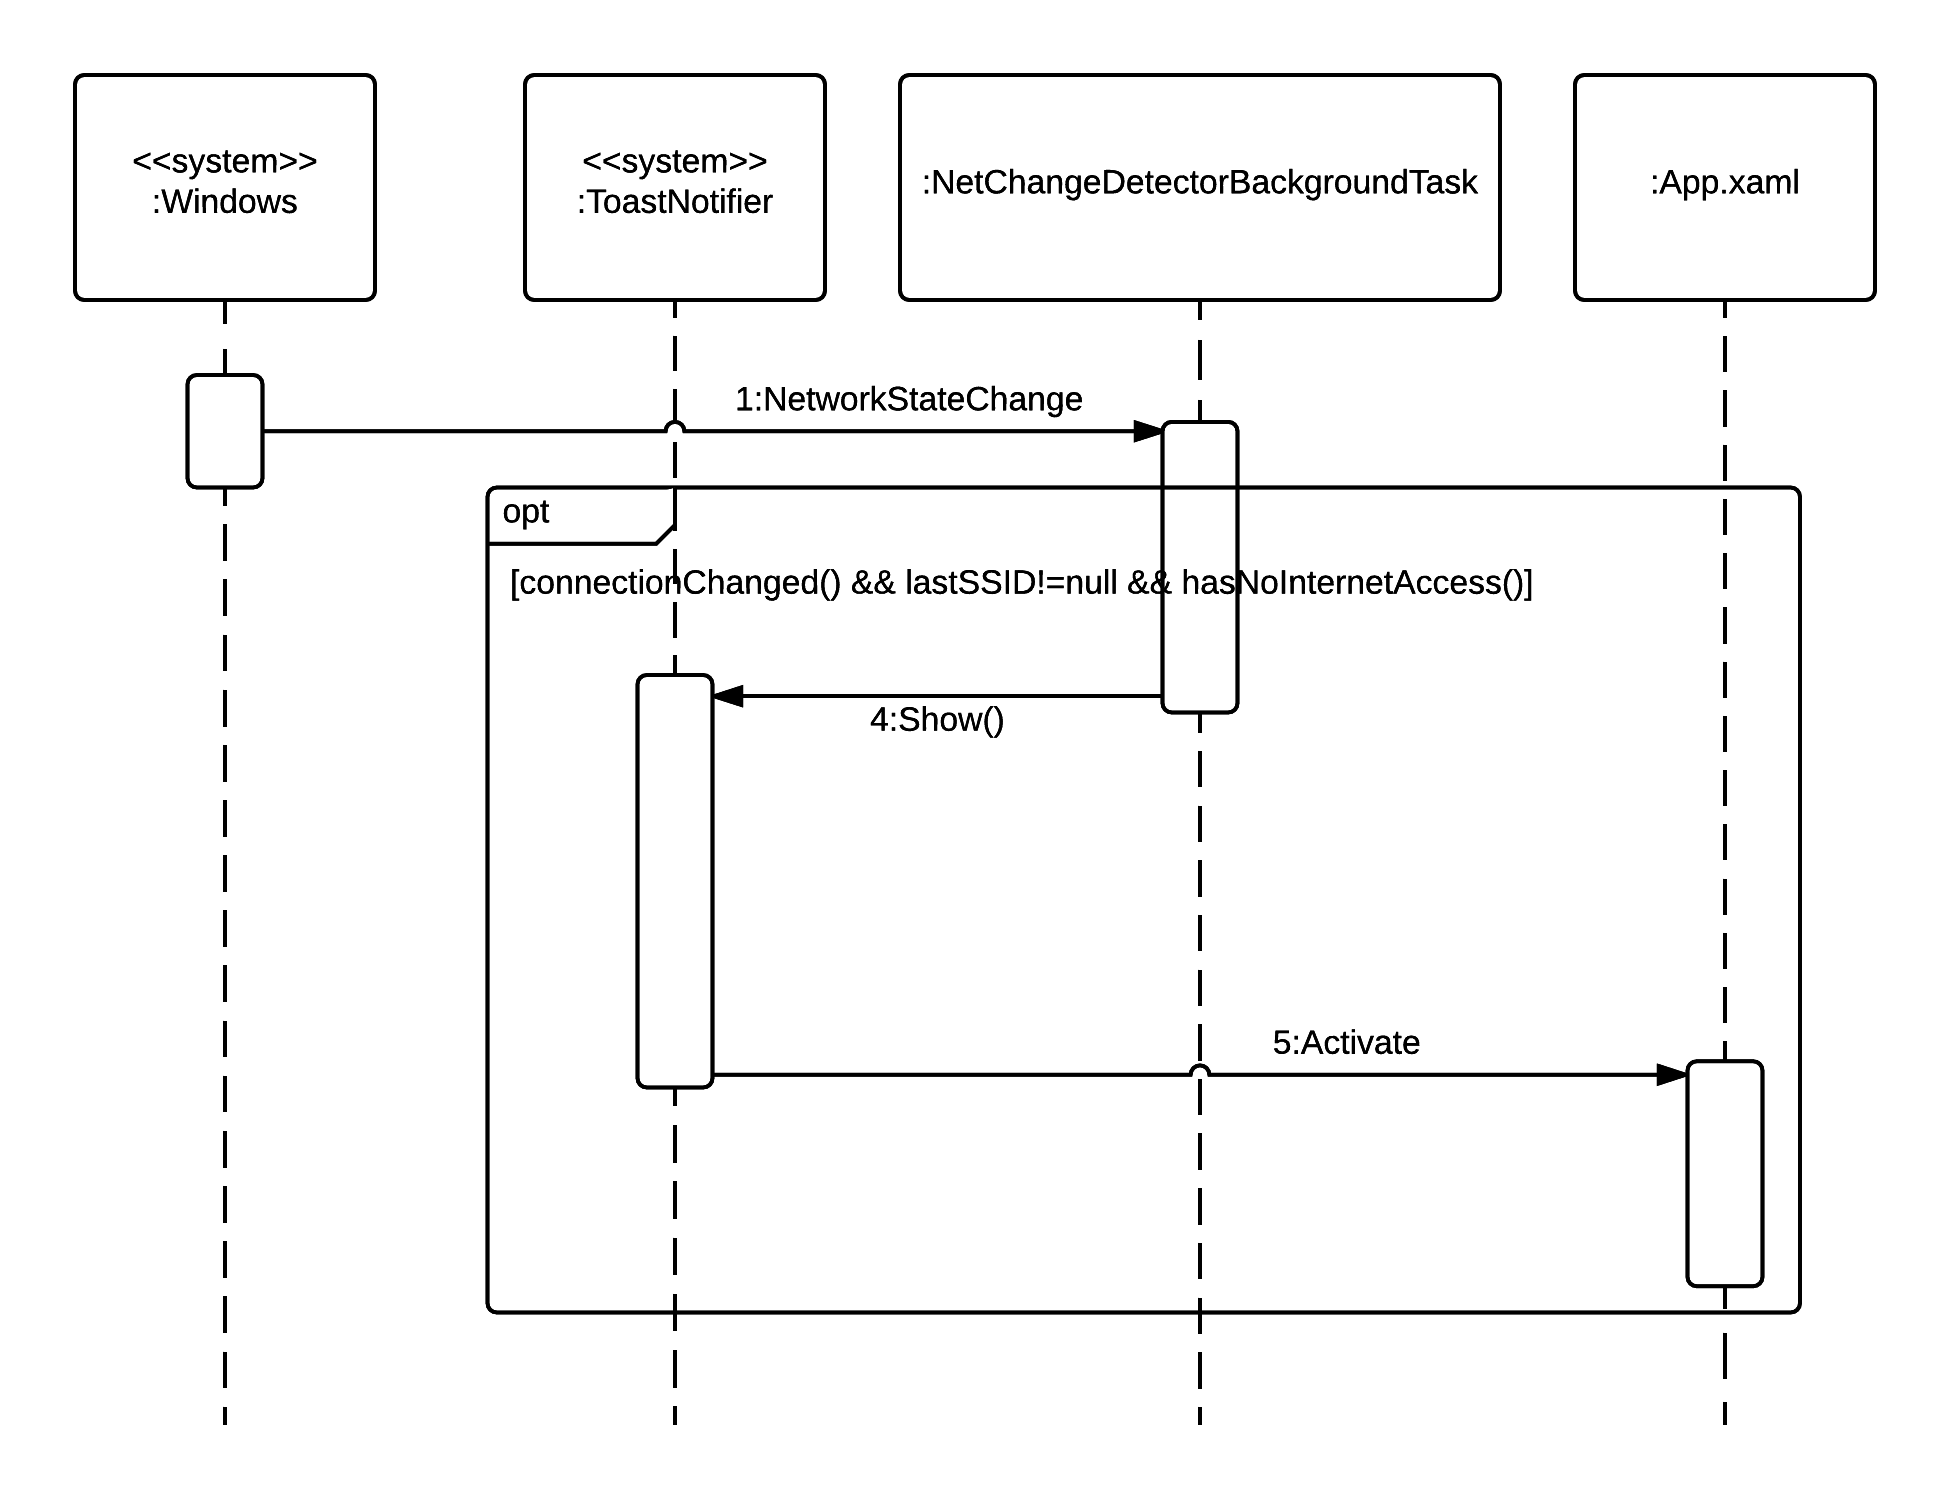
\includegraphics[scale=0.9]{SequenceDiagramNetworkDetection.png}
                            \caption[Diagram Interaksi Deteksi Jaringan.]{Diagram Interaksi Deteksi Jaringan.} 
                            \label{fig:NetworkDetectionSequenceDiagram}
                        \end{figure}
                        Gambar \ref{fig:NetworkDetectionSequenceDiagram} menjelaskan mengenai interaksi antar objek dalam perangkat lunak untuk melakukan deteksi perubahan jaringan. Interaksi yang terjadi adalah sebagai berikut:

                        \begin{enumerate}
                            \item{Saat komputer mengalami perubahan jaringan (tidak terhubung menjadi terhubung dan sebaliknya, atau terjadi perubahan \textit{cost} jaringan), \textit{trigger} NetworkStateChange akan diaktifkan oleh Windows, dan objek NetChangeDetectorBackgroundTask yang sudah didaftarkan akan menerima \textit{trigger} tersebut.}
                            \item{Jika kondisi \texttt{connectionChanged() \&\& lastSSID!=null \&\& hasNoInternetAccess()} terpenuhi, maka:}
                            \begin{enumerate}
                                \item{NetChangeDetectorBackgroundTask memerintahkan ToastNotifier untuk memunculkan notifikasi menggunakan method Show().}
                                \item{Saat user menekan tombol "Yes" pada notifikasi, App.xaml diaktivasi.}
                            \end{enumerate}
                        \end{enumerate}
                    }
                    \item{
                        {\bf Perancangan Interaksi Penciptaan Password}
                        \begin{figure}[!htb]
                            \centering
                            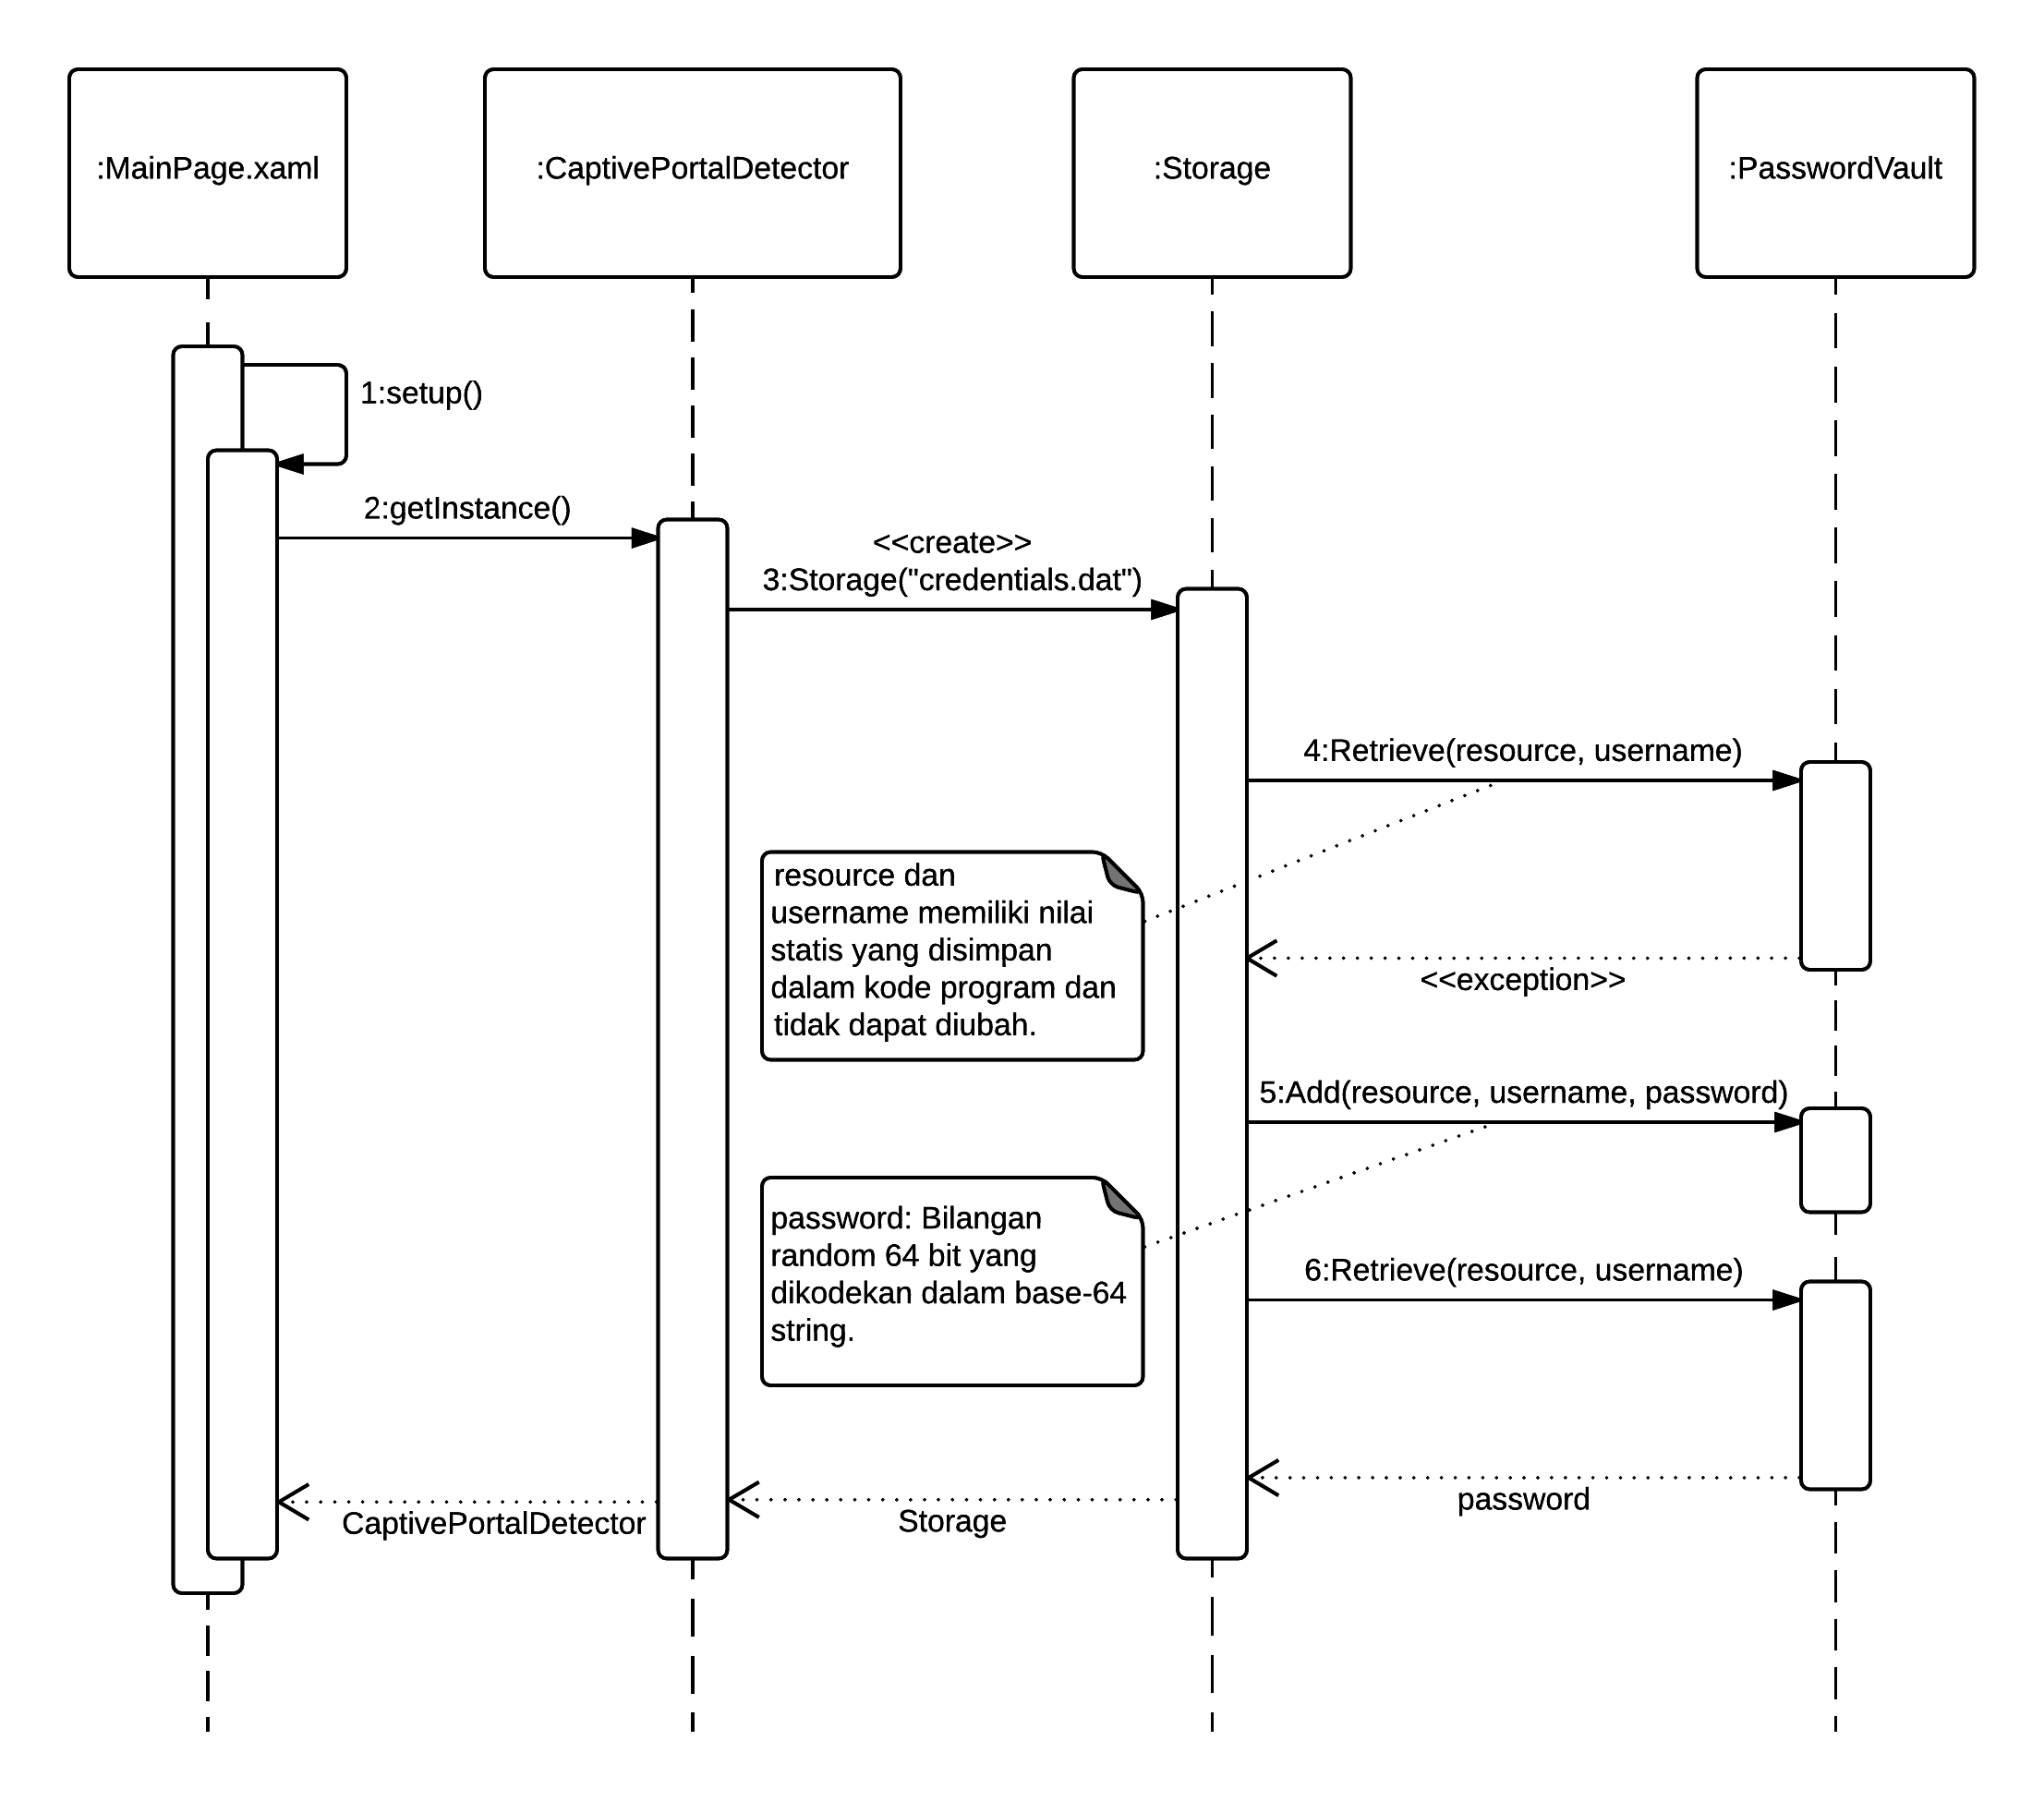
\includegraphics[scale=0.9]{SequenceDiagramPasswordGeneration.png}
                            \caption[Diagram Interaksi Penciptaan Password.]{Diagram Interaksi Penciptaan Password.} 
                            \label{fig:PasswordGenerationSequenceDiagram}
                        \end{figure}

                        Gambar \ref{fig:PasswordGenerationSequenceDiagram} menjelaskan mengenai interaksi antar objek dalam perangkat lunak untuk menciptakan password random saat perangkat lunak pertama kali dijalankan. Interaksi yang terjadi adalah sebagai berikut:

                        \begin{enumerate}
                            \item{MainPage.xaml melakukan setup().}
                            \item{MainPage.xaml memanggil metode getInstance() pada CaptivePortalDetector untuk mendapatkan \textit{instance} CaptivePortalDetector.}
                            \item{CaptivePortalDetector menciptakan objek Storage baru pada \textit{constructor}-nya.}
                            \item{Objek Storage berusaha untuk mendapatkan password dengan memangil metode Retrieve() pada objek PasswordVault, namun mendapatkan exception karena belum ada password yang disimpan.}
                            \item{Objek Storage memasukkan password baru yang diciptakan secara random menggunakan metode Add() pada PasswordVault.}
                            \item{Objek Storage memanggil metode Retrieve() kembali pada objek PasswordVault, dan mendapatkan password yang baru saja diciptakan. Setelah itu, CaptivePortalDetector mendapatkan objek Storage, dan MainPage.xaml mendapatkan \textit{instance} CaptivePortalDetector.}
                        \end{enumerate}
                    }
                    \item{
                        {\bf Perancangan Interaksi Penyimpanan Informasi Login}
                        \begin{figure}[!htb]
                            \centering
                            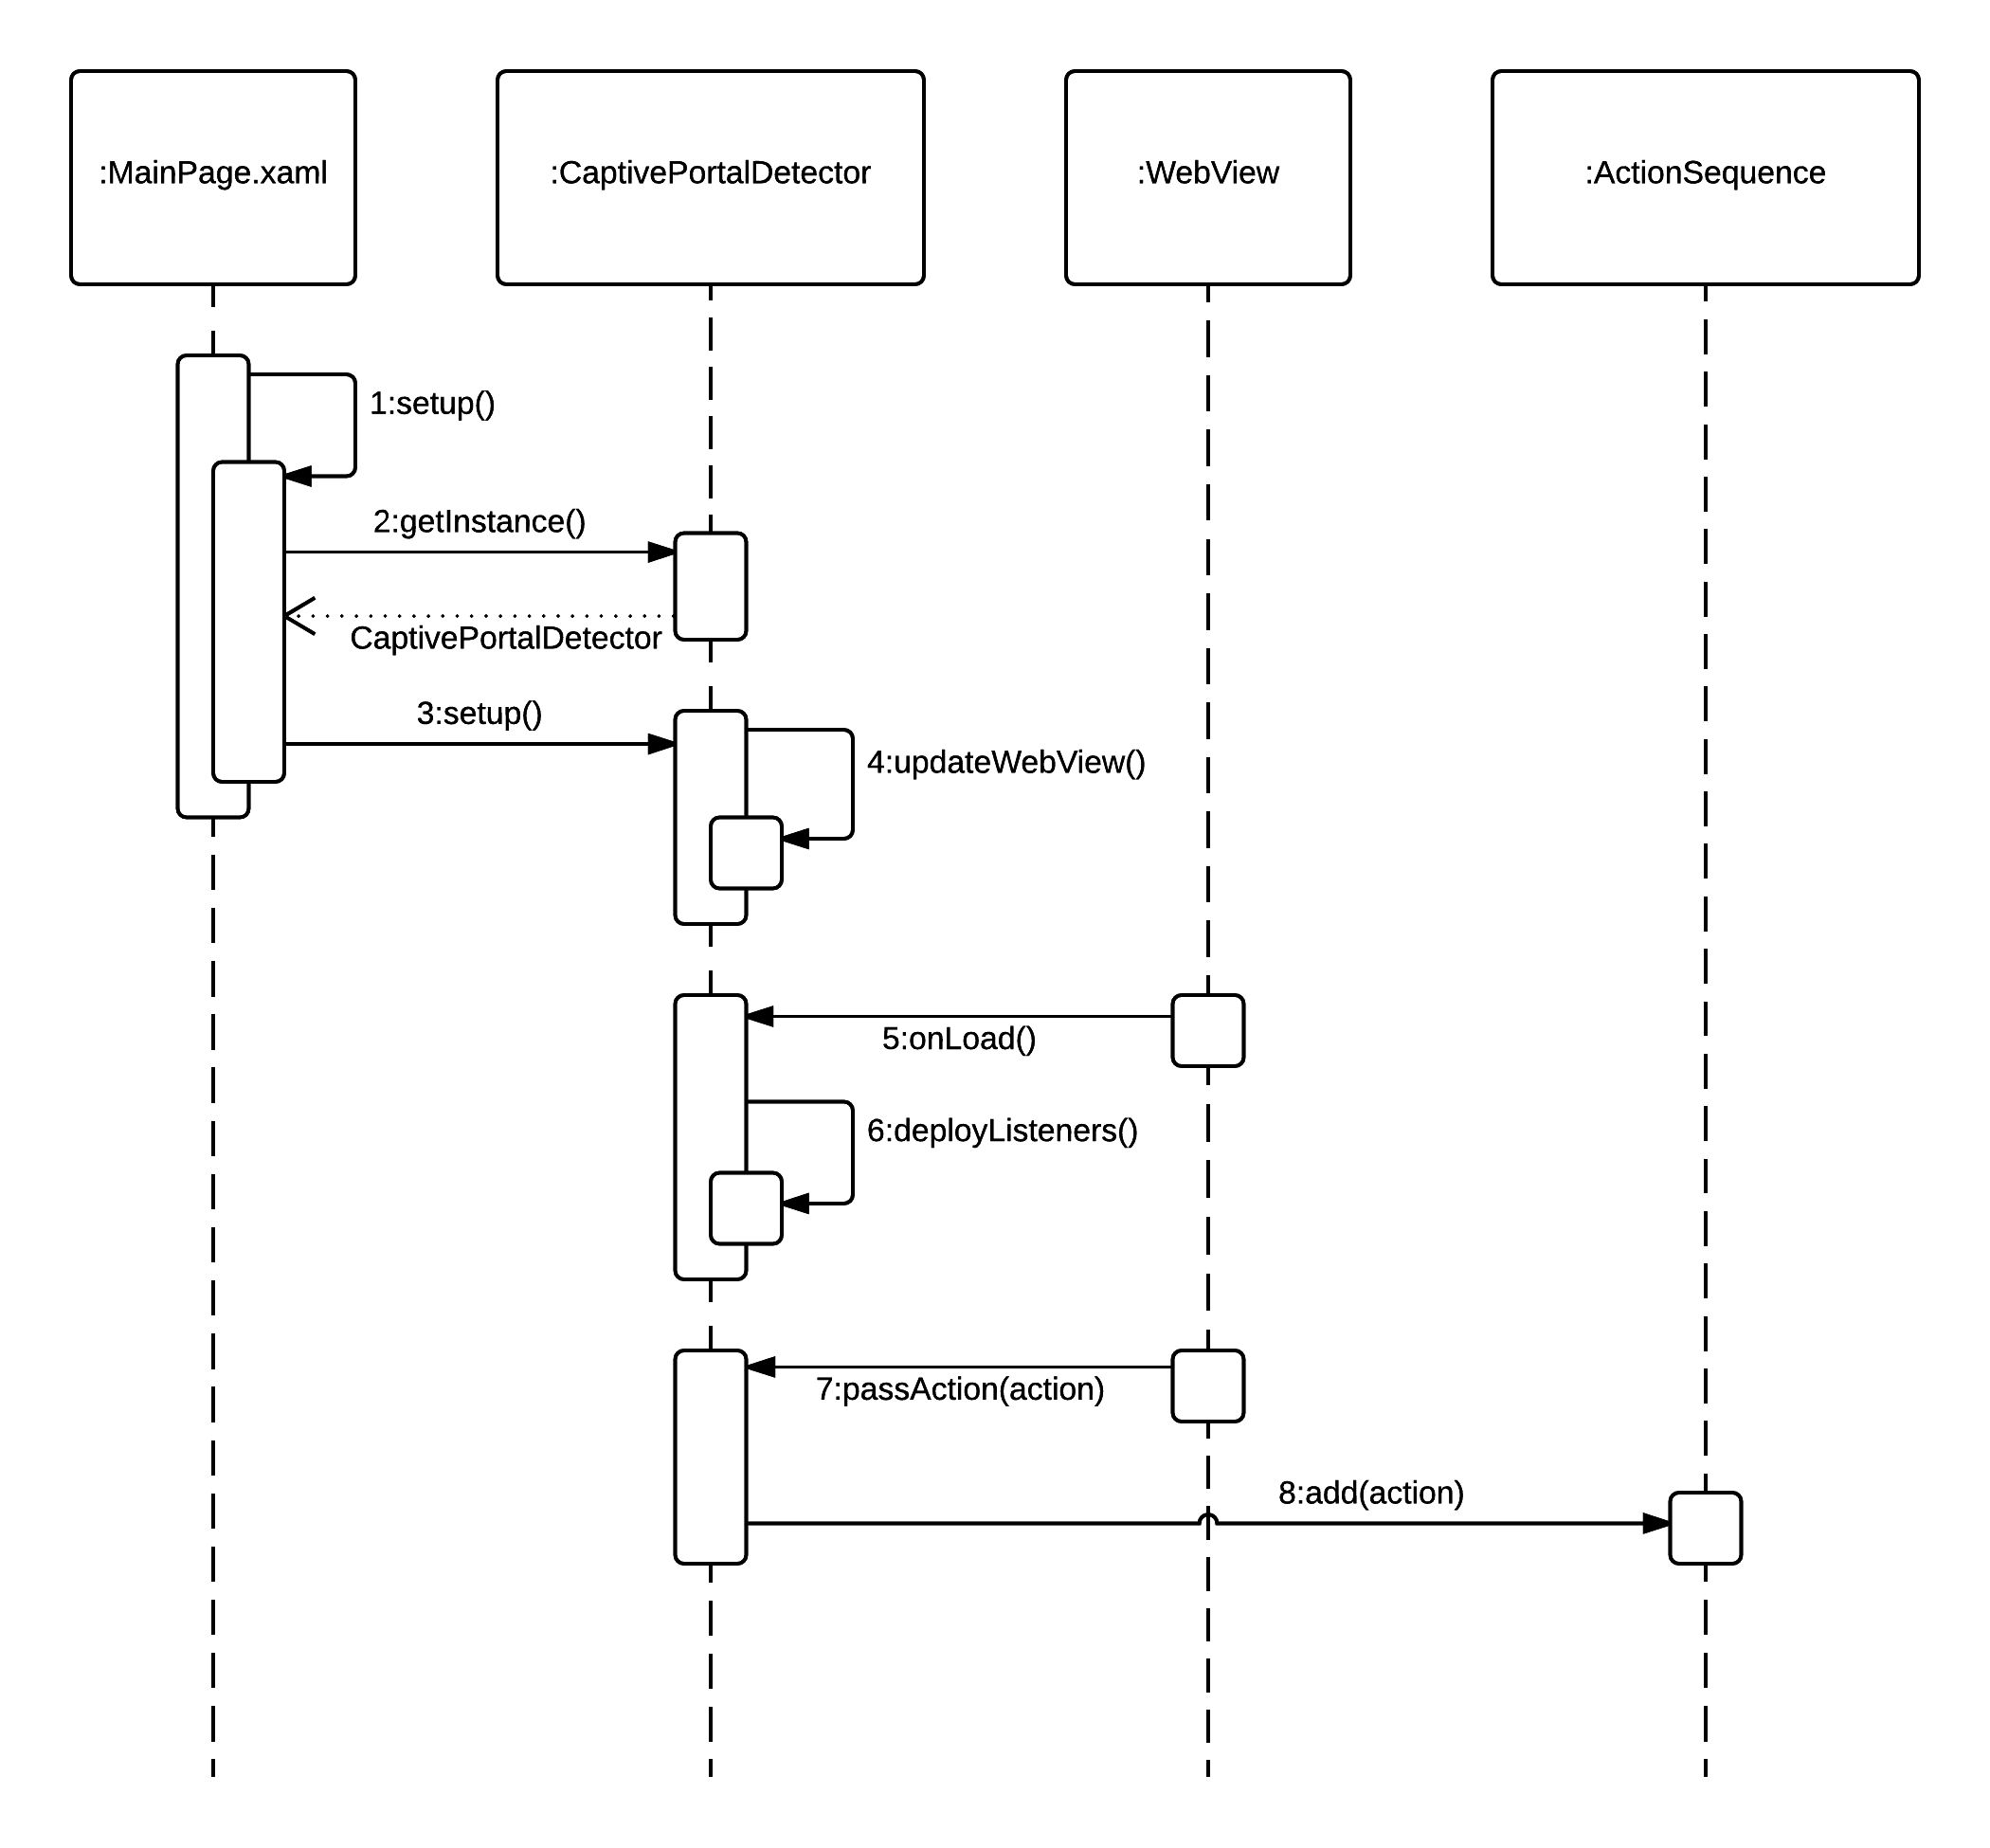
\includegraphics[scale=0.9]{SequenceDiagramLoginInformationSaving.png}
                            \caption[Diagram Interaksi Penyimpanan Informasi Login.]{Diagram Interaksi Penyimpanan Informasi Login.} 
                            \label{fig:LoginInformationSavingSequenceDiagram}
                        \end{figure}

                        Gambar \ref{fig:LoginInformationSavingSequenceDiagram} menjelaskan mengenai interaksi antar objek dalam perangkat lunak untuk menyimpan informasi login. Interaksi yang terjadi adalah sebagai berikut:

                        \begin{enumerate}
                            \item{MainPage.xaml melakukan setup().}
                            \item{MainPage.xaml memanggil metode getInstance() pada kelas CaptivePortalDetector untuk mendapatkan \textit{instance} CaptivePortalDetector. MainPage.xaml mendapatkan \textit{instance} CaptivePortalDetector.}
                            \item{MainPage.xaml memanggil metode setup() pada objek CaptivePortalDetector.}
                            \item{CaptivePortalDetector melakukan updateWebView() untuk mengarahkan WebView ke URI yang digunakan untuk melakukan deteksi koneksi internet.}
                            \item{WebView memanggil metode onLoad() pada objek CaptivePortalDetector saat halaman selesai dimuat.}
                            \item{Jika halaman tidak berisi teks "connected" (tanpa tanda petik), CaptivePortalDetector melakukan deployListeners() untuk menangkap semua \textit{event} yang mungkin dilakukan oleh pengguna pada halaman tersebut.}
                            \item{Metode passAction() dipanggil pada objek CaptivePortalDetector saat pengguna melakukan klik atau input teks untuk mengirimkan aksi yang baru saja dilakukan oleh pengguna.}
                            \item{CaptivePortalDetector memanggil metode add() pada objek ActionSequence untuk menyimpan aksi tersebut.}
                        \end{enumerate}
                    }
                \end{itemize}
            }
            \item{
                {\bf Perancangan Antarmuka}\\
                Pengguna memerlukan antarmuka untuk berinteraksi dengan perangkat lunak. Antarmuka yang diperlukan adalah:
                \begin{itemize}
                    \item{
                        {\bf Antarmuka Notifikasi}
                        \begin{figure}[!htb]
                            \centering
                            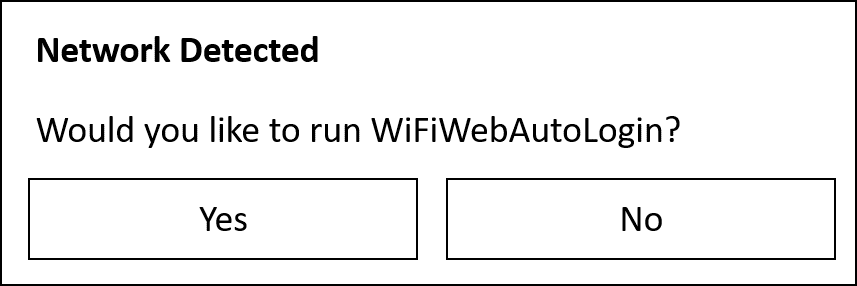
\includegraphics[scale=0.5]{UI_Notification.png}
                            \caption[Rancangan Antarmuka Notifikasi.]{Rancangan Antarmuka Notifikasi.}
                            \label{fig:RancanganAntarmukaNotifikasi}
                        \end{figure}

                        Antarmuka notifikasi muncul setiap kali terhubung dengan WiFi yang menggunakan \textit{captive portal}. Gambar \ref{fig:RancanganAntarmukaNotifikasi} menampilkan desain antarmuka notifikasi. Desain antarmuka notifikasi menggunakan desain notifikasi standar windows dengan dua tombol, "Yes" dan "No". Jika tombol "Yes" ditekan, maka notifikasi akan hilang dan aplikasi akan dijalankan. Jika tombol "No" ditekan, maka notifikasi akan hilang. Antarmuka notifikasi adalah antarmuka yang pertama kali akan muncul dalam siklus aplikasi karena kelas NetChangeDetectorBackgroundTask didaftarkan pada sistem untuk mendeteksi perubahan jaringan.
                    }
                    \item{
                        {\bf Antarmuka Message Box}
                        \begin{figure}[!htb]
                            \centering
                            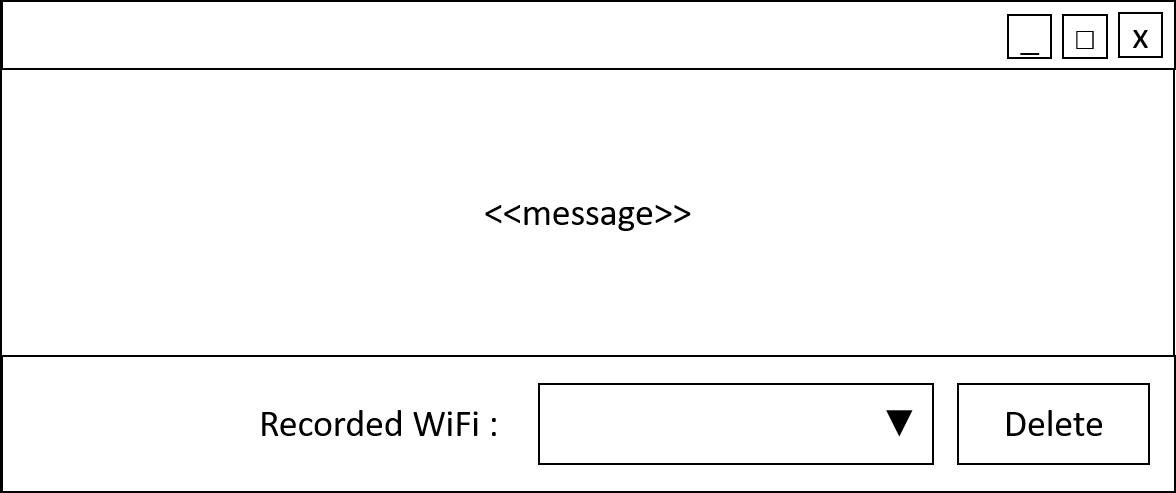
\includegraphics[scale=0.5]{UI_MessageBox.png}
                            \caption[Rancangan Antarmuka Message Box.]{Rancangan Antarmuka Message Box.}
                            \label{fig:RancanganAntarmukaMessageBox}
                        \end{figure}

                        Gambar \ref{fig:RancanganAntarmukaMessageBox} menampilkan desain antarmuka message box. Selain label untuk menaruh pesan, antarmuka ini juga memiliki \textit{selector} untuk dapat menghapus WiFi yang sudah terekam. Dengan menghapus WiFi yang terdapat pada \textit{selector} ini, pengguna dapat merekam ulang informasi login pada WiFi tersebut.
                    }
                    \item{
                        {\bf Antarmuka Web Browser}
                        \begin{figure}[!htb]
                            \centering
                            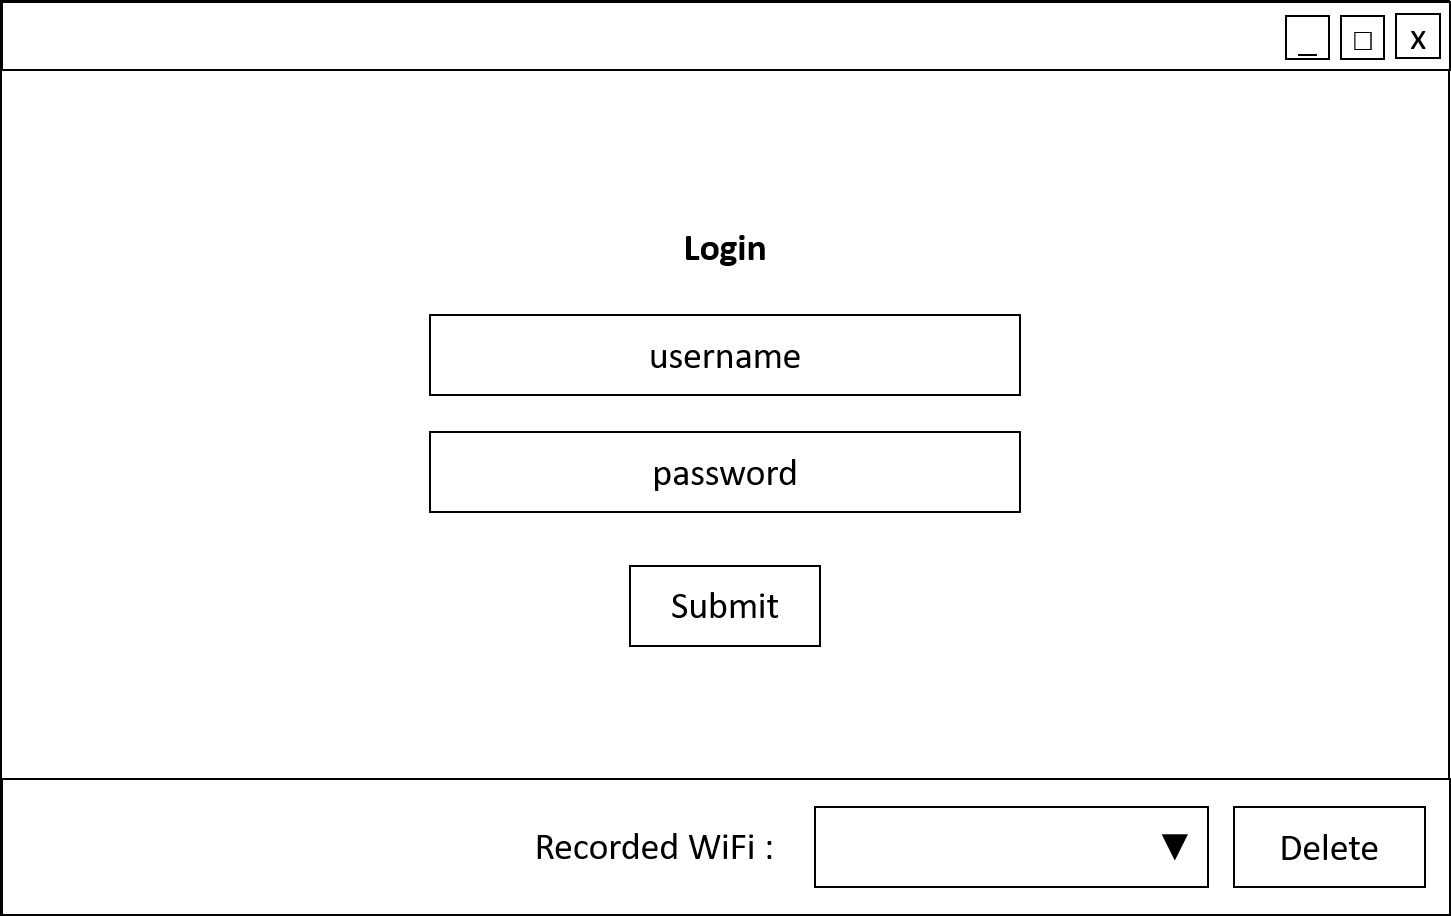
\includegraphics[scale=0.5]{UI_WebBrowser.png}
                            \caption[Rancangan Antarmuka Web Browser.]{Rancangan Antarmuka Web Browser.}
                            \label{fig:RancanganAntarmukaWebBrowser}
                        \end{figure}

                        Gambar \ref{fig:RancanganAntarmukaWebBrowser} menampilkan desain antarmuka web browser. Antarmuka ini digunakan untuk menampilkan halaman web yang berkaitan dengan login \textit{captive portal}. Pada antarmuka inilah aksi pengguna akan direkam secara otomatis. Selain itu, pada antarmuka ini terdapat komponen yang sama dengan antarmuka message box, yaitu komponen \textit{selector} untuk menghapus SSID WiFi yang sudah terekam.
                    }
                \end{itemize}
                
            }
        \end{itemize}

		\item  Melakukan pengujian terhadap perangkat lunak untuk menghasilkan perbaikan teradap perangkat
lunak tersebut.\\
		{\bf status :} Ada sejak rencana kerja skripsi. \\
		{\bf hasil :} Setelah dilakukan implementasi pertama, ditemukan beberapa masalah yang membuat rancangan perangkat lunak tidak dapat sepenuhnya didasarkan pada hasil analisis, di antaranya:

            \begin{itemize}
                \item{Fungsi window.external.notify tidak berperilaku sebagaimana yang diperkirakan. Fungsi ini diharapkan dapat dipanggil secara langsung di dalam kode javascript, namun ternyata tidak bisa. Setiap halaman yang ingin memanfaatkan fungsi ini harus didaftarkan pada Package.appxmanifest. Metode yang digunakan untuk mendapatkan hasil yang sama dengan fungsi yang diberikan oleh window.external.notify adalah dengan menggunakan kelas bertipe RuntimeComponent yang diizinkan untuk dapat diakses oleh JavaScript pada WebView. Kelas ini adalah ScriptNotifyHandler pada gambar \ref{fig:DetailedClassDiagram}.}
                \item{Fungsi window.open dan fungsi open tidak dapat dijalankan secara otomatis sehingga popup tidak muncul. Metode yang digunakan untuk mendapatkan hasil yang sama dari yang direncanakan sebelumnya adalah dengan melakukan \textit{override} fungsi window.open dan fungsi open pada saat halaman selesai dimuat, dan mengubungkannya dengan kelas ScriptNotifyHandler. Akan tetapi, metode ini masih kurang memadai karena kode JavaScript yang memanggil fungsi-fungsi tersebut pada saat halaman dimuat akan dieksekusi sebelum \textit{override} terjadi.}
            \end{itemize}

            Perancangan yang sudah dibuat merupakan hasil revisi dari pengujian ini.

		\item Melakukan pengujian (dan eksperimen) yang melibatkan responden untuk menilai hasil simulasi secara kualitatif\\
		{\bf status :} Ada sejak rencana kerja skripsi. Namun responden tidak dibutuhkan untuk keperluan pengujian.\\
		{\bf hasil :} Pengujian dibagi menjadi 2 bagian, yaitu pengujian fungsional dan pengujian eksperimental.
        \begin{itemize}
            \item{
                {\bf Pengujian Fungsional}\\
                Pengujian fungsional dilakukan pada jaringan WiFi di kost di jalan Ciumbuleuit nomor 149, Bandung, dengan SSID "C149Net".
                \begin{itemize}
                    \item{
                        {\bf Rencana Pengujian Fungsional}\\
                        Pengujian fungsional dilakukan menggunakan teknik \textit{black box}. Pengujian fungsional dilakukan untuk memastikan fungsi-fungsi utama dalam perangkat lunak sudah berjalan dengan baik. Fungsi-fungsi yang akan diuji mencakupi:

                        \begin{itemize}
                            \item{Deteksi perubahan jaringan.}
                            \item{Deteksi \textit{captive portal}.}
                            \item{Login otomatis.}
                        \end{itemize}

                        Setiap fungsi yang diuji diberikan kasus pengujian positif dan pengujian negatif.
                    }
                    \item{
                        {\bf Hasil Pengujian Fungsional}\\
                        Hasil-hasil pengujian fungsional adalah sebagai berikut:

                        \begin{itemize}
                            \item{
                                \textbf{Pengujian deteksi perubahan jaringan}
                                
                                \begin{itemize}
                                    \item{
                                        \textbf{Pengujian positif}\\
                                        \textbf{Kasus}: Menghubungkan komputer dengan WiFi yang terhubung dengan \textit{captive portal}.\\
                                        \textbf{Hasil yang diharapkan}: Muncul notifikasi.\\
                                        \textbf{Hasil yang didapatkan}: Muncul notifikasi "Network Detected" dengan pesan "Would you like to run WiFiWebAutoLogin?".\\
                                        \textbf{Kesimpulan}: Fungsi berjalan sesuai harapan.
                                    }
                                    \item{
                                        \textbf{Pengujian negatif}\\
                                        \textbf{Kasus}: Menghubungkan komputer dengan WiFi yang tidak terhubung dengan \textit{captive portal}.\\
                                        \textbf{Hasil yang diharapkan}: Tidak muncul notifikasi apapun.\\
                                        \textbf{Hasil yang didapatkan}: Tidak muncul notifikasi apapun.\\
                                        \textbf{Kesimpulan}: Fungsi berjalan sesuai harapan.
                                    }
                                \end{itemize}
                            }
                            \item{
                                \textbf{Pengujian deteksi \textit{captive portal}}
                                
                                \begin{itemize}
                                    \item{
                                        \textbf{Pengujian positif}\\
                                        \textbf{Kasus}: Menghubungkan komputer dengan WiFi yang terhubung dengan \textit{captive portal} dan menekan tombol "Yes" pada notifikasi.\\
                                        \textbf{Hasil yang diharapkan}: Muncul halaman login.\\
                                        \textbf{Hasil yang didapatkan}: Muncul halaman login \textit{captive portal}.\\
                                        \textbf{Kesimpulan}: Fungsi berjalan sesuai harapan.
                                    }
                                    \item{
                                        \textbf{Pengujian negatif}\\
                                        \textbf{Kasus}: Menghubungkan komputer dengan WiFi yang tidak terhubung dengan \textit{captive portal} maupun internet dan menekan tombol "Yes" pada notifikasi\\
                                        \textbf{Hasil yang diharapkan}: Muncul pesan \textit{timeout}.\\
                                        \textbf{Hasil yang didapatkan}: Muncul pesan "Operation timeout. Check your network connection.".\\
                                        \textbf{Kesimpulan}: Fungsi berjalan sesuai harapan.
                                    }
                                \end{itemize}
                            }
                            \item{
                                \textbf{Pengujian login otomatis}
                                
                                \begin{itemize}
                                    \item{
                                        \textbf{Pengujian positif}\\
                                        \textbf{Kasus}: Menghubungkan komputer dengan WiFi yang terhubung dengan \textit{captive portal} yang sudah pernah dijalankan login secara manual.\\
                                        \textbf{Hasil yang diharapkan}: Muncul pesan "Connected.".\\
                                        \textbf{Hasil yang didapatkan}: Muncul pesan "Executing recorded actions...", lalu setelah beberapa saat, muncul pesan "Connected.".\\
                                        \textbf{Kesimpulan}: Fungsi berjalan sesuai harapan.
                                    }
                                    \item{
                                        \textbf{Pengujian negatif}\\
                                        \textbf{Kasus}: Menghubungkan komputer dengan WiFi yang terhubung dengan \textit{captive portal} yang belum pernah dijalankan login secara manual.\\
                                        \textbf{Hasil yang diharapkan}: Muncul halaman login.\\
                                        \textbf{Hasil yang didapatkan}: Muncul halaman login \textit{captive portal}.\\
                                        \textbf{Kesimpulan}: Fungsi berjalan sesuai harapan.
                                    }
                                \end{itemize}
                            }
                        \end{itemize}
                    }
                \end{itemize}
            }
            \item{
                {\bf Pengujian Eksperimental}\\
                Pengujian eksperimental dilakukan untuk memeriksa apakah perangkat lunak dapat berjalan pada beragam \textit{captive portal}.
                \begin{itemize}
                    \item{
                        {\bf Rencana Pengujian Eksperimental}\\
                        Pengujian eksperimental dilakukan pada \textit{captive portal} pada jaringan WiFi dengan SSID:

                        \begin{itemize}
                            \item{\textit{C149Net} pada kost di jalan Ciumbuleuit nomor 149, Bandung.}
                            \item{\textit{Starbucks@wifi.id} pada Starbucks Dipatiukur, Bandung.}
                            \item{\textit{wifi.id} pada Starbucks Dipatiukur, Bandung.}
                            \item{\textit{UNPAR9} pada gedung 10 Universitas Katolik Parahyangan, Bandung.}
                            \item{\textit{FTIS.cisco} pada gedung 9 Universitas Katolik Parahyangan, Bandung.}
                        \end{itemize}
                    }
                    \item{
                        {\bf Hasil Pengujian Eksperimental}\\
                        Hasil pengujian eksperimental akan dijelaskan untuk setiap SSID yang diuji. Penjelasan berupa narasi hasil yang didapatkan berdasarkan langkah-langkah yang sama dengan pengujian fungsional \textit{black box}.
                        \begin{itemize}
                            \item{
                                {\bf Hasil Pengujian WiFi C149Net}\\
                                Pengujian pada WiFi dengan SSID C149Net yang berlokasi pada kost di jalan Ciumbuleuit nomor 149, Bandung, mendapatkan hasil sesuai harapan. Notifikasi muncul pada saat WiFi pertama kali terhubung. Halaman login muncul setelah tombol "Yes" pada notifikasi ditekan. Setelah memasukkan \textit{username} dan \textit{password}, pesan "Connected." muncul. Jika informasi login sudah tersimpan, pesan "Connected." akan langsung muncul setelah menekan tombol "Yes" pada notifikasi.
                            }
                            \item{
                                {\bf Hasil Pengujian WiFi Starbucks@wifi.id}\\
                                Pengujian pada WiFi dengan SSID Starbucks@wifi.id yang berlokasi pada Starbucks Dipatiukur, Bandung, mendapatkan hasil sesuai harapan. Notifikasi muncul pada saat WiFi pertama kali terhubung. Halaman \textit{captive portal} muncul setelah tombol "Yes" pada notifikasi ditekan. Setelah menekan tombol "continue" pada halaman tersebut, lalu menekan tombol "lanjutkan" pada halaman selanjutnya, pesan "Connected." muncul. Jika informasi login sudah tersimpan, pesan "Connected." akan langsung muncul setelah menekan tombol "Yes" pada notifikasi.
                            }
                            \item{
                                {\bf Hasil Pengujian WiFi wifi.id}\\
                                Pengujian pada WiFi dengan SSID wifi.id yang berlokasi pada Starbucks Dipatiukur, Bandung, mendapatkan hasil yang tidak sesuai harapan. Notifikasi muncul pada saat WiFi pertama kali terhubung. Halaman login muncul setelah tombol "Yes" pada notifikasi ditekan. Akan tetapi, login tidak dapat dilakukan karena perlu membeli voucher setiap kali ingin melakukan login.
                            }
                            \item{
                                {\bf Hasil Pengujian WiFi UNPAR9}\\
                                Pengujian pada WiFi dengan SSID UNPAR9 yang berlokasi pada gedung 10 Universitas Katolik Parahyangan, Bandung, mendapatkan hasil yang tidak sesuai harapan. Notifikasi muncul pada saat WiFi pertama kali terhubung. Halaman login muncul setelah tombol "Yes" pada notifikasi ditekan. Setelah login dilakukan, proses terhenti pada halaman \texttt{https://portal.unpar.ac.id/home}. Hal ini dikarenakan WiFi di Universitas Katolik Parahyangan menggunakan CAS\footnote{\textit{Central Authorization Service}}. Selain itu, CAS ini menggunakan \textit{pop-up} untuk menampilkan halaman \texttt{https://wireless.unpar.ac.id/status} dan halaman tersebut adalah halaman yang membuka popup yang menuju ke halaman tujuan. WebView pada UWP tidak memperbolehkan pemanggilan fungsi open(), window.open(), el.click() dan form.submit() yang bukan merupakan aksi langsung oleh pengguna. \textit{Override} tiap fungsi tersebut dimungkinkan setelah halaman selesai dimuat, namun itu berarti fungsi hasil \textit{override} tidak akan digunakan jika fungsi tersebut dipanggil pada saat halaman pertama kali dimuat. Hal ini mencakup \textit{onload event} dan script yang dipanggil langsung pada \textit{script tag} baik pada \textit{body} maupun \textit{head}.
                            }
                            \item{
                                {\bf Hasil Pengujian WiFi FTIS.cisco}\\
                                Pengujian pada WiFi dengan SSID FTIS.cisco yang berlokasi pada gedung 9 Universitas Katolik Parahyangan, Bandung, mendapatkan hasil yang tidak sesuai harapan. Hal ini terjadi karena WiFi ini merupakan jaringan internal Fakultas Teknologi dan Sains yang menggunakan jaringan WiFi Universitas Katolik Parahyangan untuk akses internet. Proses terhenti pada halaman yang sama dengan WiFi UNPAR9, yaitu pada halaman \texttt{https://portal.unpar.ac.id/home}. Penyebab terjadinya hal ini juga sama dengan yang terjadi pada WiFi UNPAR9.
                            }
                        \end{itemize}
                    }
                \end{itemize}
            }
        \end{itemize}
        
        \item Membuat kesimpulan dari hasil penelitian dan saran untuk penelitian selanjutnya.\\
		{\bf status :} Ada sejak rencana kerja skripsi.\\
		{\bf hasil :} Kesimpulan dan saran yang dihasilkan dari penelitian ini adalah:
        \begin{itemize}
            \item{
                {\bf Kesimpulan}
                \begin{itemize}
                    \item{Implementasi perangkat lunak untuk melakukan login otomatis pada \textit{captive portal} berhasil dilakukan walaupun memiliki keterbatasan tidak dapat melakukan login otomatis jika \textit{captive portal} bergantung pada pop-up untuk mengakses halaman tujuan.}
                    \item{\textit{Username} dan \textit{password} sudah disimpan secara aman dalam file yang dienkripsi menggunakan kunci yang diciptakan secara random per aplikasi.}
                    \item{SSID, uri, dan konten \textit{tag} head adalah informasi yang dibutuhkan untuk membedakan antar halaman pada setiap \textit{captive portal}.}
                \end{itemize}
            }
            \item{
                {\bf Saran}\\
                Saran dari peneliti yang dapat dilakukan untuk mengembangkan penelitian ini adalah gunakan \textit{platform} lain selain UWP, seperti Windows Form, Java, Android, atau iOS. Hal ini dapat dilakukan untuk menghindari keterbatasan WebView pada UWP dalam menangani pop-up. Jika ingin tetap menggunakan UWP, maka penerus penelitian ini harus menciptakan WebView sendiri. Hal ini dapat dilakukan menggunakan Canvas yang sudah disediakan oleh UWP dan menggabungkannya dengan teknologi-teknologi yang sudah ada seperti webkit atau gecko.
            }
        \end{itemize}

		\item Menulis dokumen skripsi.\\
		{\bf status :} Ada sejak rencana kerja skripsi.\\
		{\bf hasil :} Sudah dikerjakan sampai dengan bab 6 (Kesimpulan dan Saran)\footnote{https://github.com/yohanesmario/Skripsi/raw/master/doc/DokumenSkripsi/main.pdf}.

	\end{enumerate}

\pagebreak

\section{Pencapaian Rencana Kerja\footnote{Terdapat kesalahan pada dokumen rencana kerja terdahulu di mana terdapat 8 poin rencana kerja, sementara hanya tertera 7 poin pada tabel rencana kerja. Poin-poin rencana kerja yang benar adalah yang ada pada dokumen ini.}}

Persentase penyelesaian skripsi sampai dengan dokumen ini dibuat dapat dilihat pada tabel berikut :

\begin{center}
  \begin{tabular}{ | c | c | c | c | l | c |}
    \hline
    1*  & 2*(\%) & 3*(\%) & 4*(\%) &5* &6*(\%)\\ \hline \hline
    1   & 5  & 5  &  &  & 5 \\ \hline
    2   & 10 & 10  &   &  & 10 \\ \hline
    3   & 15  & 10  & 5 & {\footnotesize kaji ulang singkat kebutuhan pada S2}  & 15  \\ \hline
    4   & 10  &  & 10 &  & 10 \\ \hline
    5   & 15  &   & 15 & & 15 \\ \hline
    6   & 5 &   & 5  & & 5 \\ \hline
    7   & 10 &   & 10  & & 10 \\ \hline
    8   & 30  & 15  & 15 & {\footnotesize sebagian bab 1 dan 2, serta bagian awal analisis di S1} & 30 \\ \hline
    Total  & 100  & 40  & 60 &  & 100\\ \hline
                          \end{tabular}
\end{center}

Keterangan (*)\\
1 : Bagian pengerjaan Skripsi (nomor disesuaikan dengan detail pengerjaan di bagian 5)\\
2 : Persentase total \\
3 : Persentase yang akan diselesaikan di Skripsi 1 \\
4 : Persentase yang akan diselesaikan di Skripsi 2 \\
5 : Penjelasan singkat apa yang dilakukan di S1 (Skripsi 1) atau S2 (skripsi 2)\\
6 : Persentase yang sidah diselesaikan sampai saat ini

%\section{Kendala yang dihadapi}
%%TULISKAN BAGIAN INI JIKA DOKUMEN ANDA TIPE A ATAU C
%Kendala - kendala yang dihadapi selama mengerjakan skripsi :
%\begin{itemize}
	%\item Terlalu banyak melakukan prokratinasi
	%\item Terlalu banyak godaan berupa hiburan (game, film, dll)
	%\item Skripsi diambil bersamaan dengan kuliah ASD karena selama 5 semester pertama kuliah tersebut sangat dihindari dan tidak diambil, dan selama 4 semester terakhir kuliah tersebut selalu mendapat nilai E
	%\item Mengalami kesulitan pada saat sudah mulai membuat program komputer karena selama ini selalu dibantu teman
%\end{itemize}

\vspace{1cm}
\centering Bandung, \tanggal\\
\vspace{2cm} \nama \\ 
\vspace{1cm}

Menyetujui, \\
\ifdefstring{\jumpemb}{2}{
\vspace{1.5cm}
\begin{centering} Menyetujui,\\ \end{centering} \vspace{0.75cm}
\begin{minipage}[b]{0.45\linewidth}
% \centering Bandung, \makebox[0.5cm]{\hrulefill}/\makebox[0.5cm]{\hrulefill}/2013 \\
\vspace{2cm} Nama: \pembA \\ Pembimbing Utama
\end{minipage} \hspace{0.5cm}
\begin{minipage}[b]{0.45\linewidth}
% \centering Bandung, \makebox[0.5cm]{\hrulefill}/\makebox[0.5cm]{\hrulefill}/2013\\
\vspace{2cm} Nama: \pemB \\ Pembimbing Pendamping
\end{minipage}
\vspace{0.5cm}
}{
% \centering Bandung, \makebox[0.5cm]{\hrulefill}/\makebox[0.5cm]{\hrulefill}/2013\\
\vspace{2cm} Nama: \pembA \\ Pembimbing Tunggal
}

\end{document}

